\documentclass{report}
\usepackage[spanish]{babel}
\usepackage[utf8]{inputenc}
\usepackage{graphicx, longtable, float}

\begin{document}
    \begin{titlepage}
        \centering
        
\includegraphics[width=0.6\textwidth]{./img/portada/logo.jpg}\\
        \vspace{1cm}
        \LARGE Análisis y Diseño de Sistemas de Información\\
        \vspace{0.5cm}
        \Large Ingeniería Informática de Gestión y Sistemas de Información\\
        \vspace{3cm}
        \Huge Biblioteca\\
        \vspace{2.5cm}
        \Large Autores:\\
        \vspace{0.2cm}
        \large Xabier Gabiña Barañano\\
        \large Janire Veganzones García\\
        \large Ainhize Martinez Duran\\
        \large Javier Criado Garcia\\
        \large Kepa Reches Urrutia\\
        \large Jon Valdes Granado\\
        \large Mohammed El Basri Dehbi\\
        \vfill
        \today
    \end{titlepage}

    \tableofcontents
    \chapter{Changelog}
        \section{Versión 1 (2023-10-08)}
            \begin{itemize}
                \item Añadido caso de uso general.
                \item Añadidos los casos de uso extendidos.
            \end{itemize}  
        \section{Versión 2 (2023-10-22)}
            \begin{itemize}
                \item Añadido modelo de dominio.
                \item Modificado el caso de uso general.
                \item Modificados los casos de uso extendidos.
            \end{itemize}
    \chapter{Introducción}
    En un mundo cada vez más digitalizado, las bibliotecas modernas están buscando formas innovadoras de adaptarse a las necesidades cambiantes de sus usuarios. La biblioteca que nos ocupa se encuentra en este proceso de transformación, reconociendo la importancia de expandir sus servicios en línea y brindar a sus usuarios una experiencia más enriquecedora y conectada. Para llevar a cabo esta ambiciosa misión, han solicitado la colaboración de nuestro equipo de desarrollo.\\
    En su estado actual, la biblioteca cuenta con un servicio web que permite a los usuarios consultar su extenso catálogo de libros. Además, ofrece un apartado de usuarios que pueden acceder a una sección privada. Sin embargo, esta plataforma carece de funcionalidades adicionales que pueden mejorar significativamente la experiencia de los usuarios y promover una mayor interacción entre ellos.\\
    En este proyecto, nuestro objetivo es expandir y mejorar el servicio web de la biblioteca, dotándolo de una serie de funcionalidades clave. Estas nuevas características incluyen la gestión de reservas, la capacidad de dejar reseñas y comentarios en los libros, la creación de una red de amigos entre los usuarios, la introducción de un rol de administrador con capacidades de gestión, la implementación de foros para discusión y la incorporación de sistemas de recomendación, tanto basados en el historial de lecturas como en la afinidad de intereses entre usuarios.\\
    A lo largo de este documento, exploraremos en detalle cada una de estas funcionalidades, presentando soluciones técnicas y estratégicas para su implementación. Este proyecto representa una emocionante oportunidad para ayudar a la biblioteca a evolucionar y brindar un servicio en línea más completo y enriquecedor a su comunidad de usuarios ávidos de conocimiento y lectura.\\
    \chapter{Casos de Uso}
        \section{General}
            \begin{figure}[H]
                \centering
                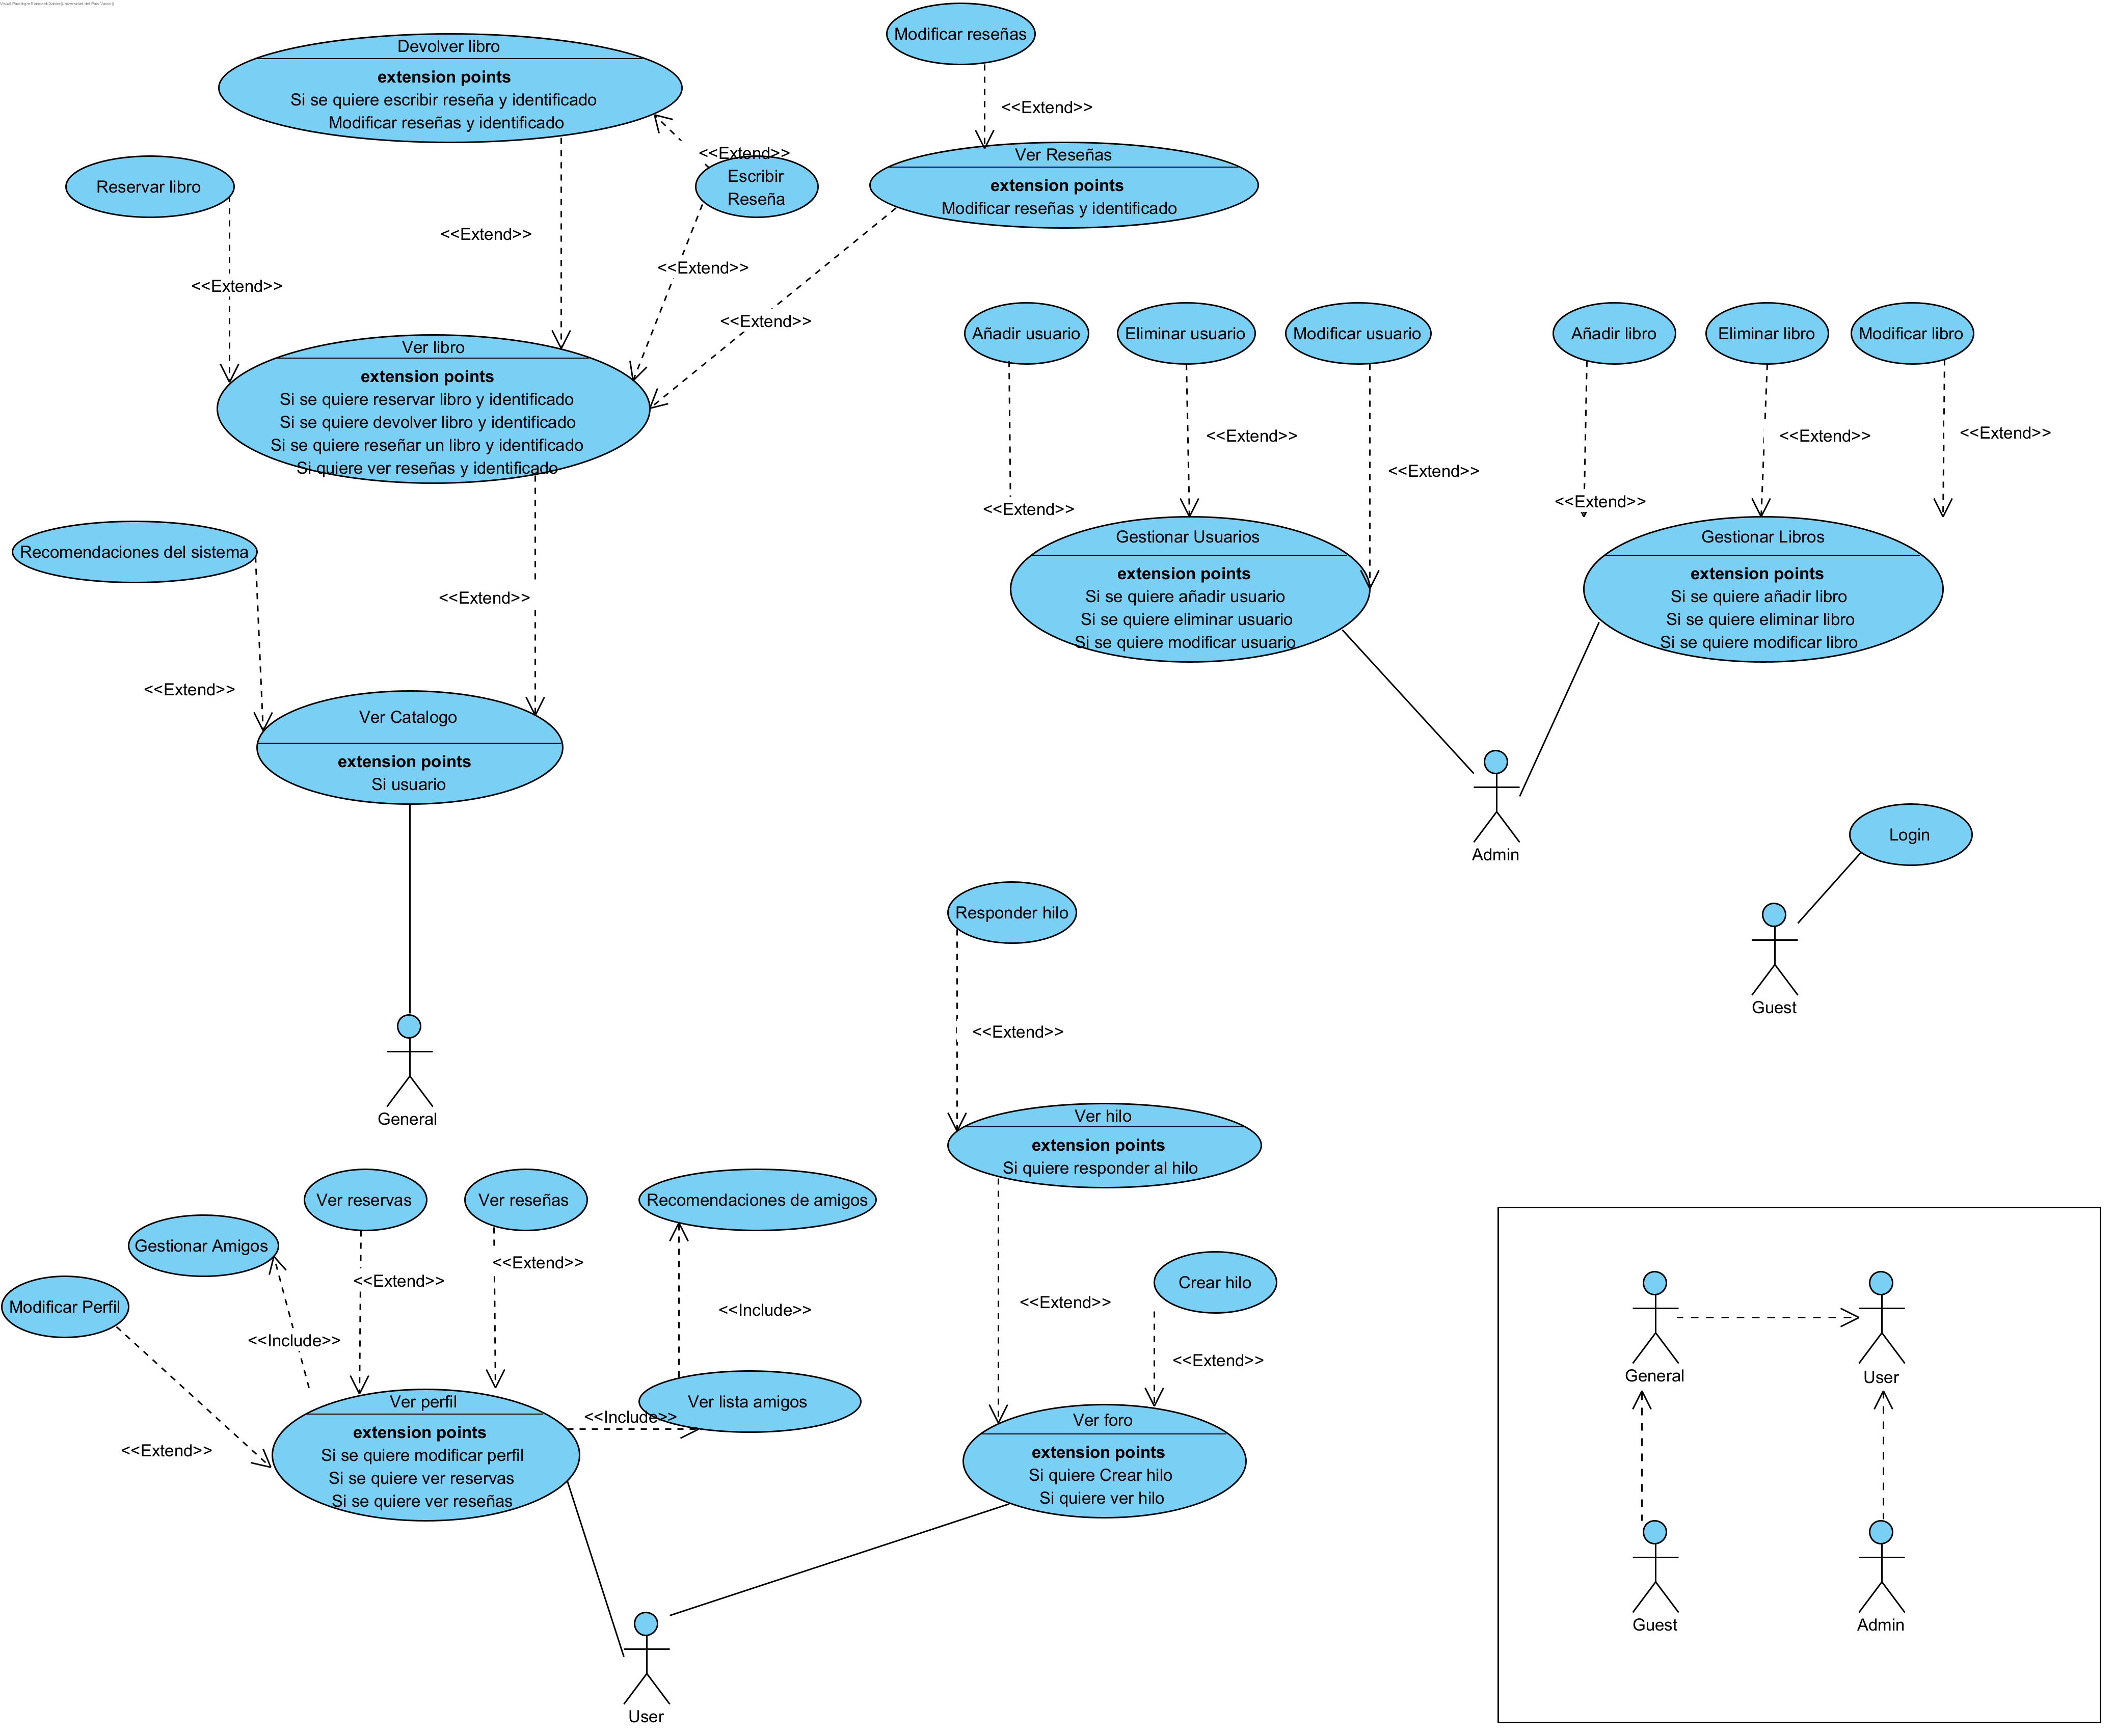
\includegraphics[scale=0.3]{img/casos_uso/General.png}
                \caption{Diagrama de casos de uso general}
            \end{figure}
        \clearpage
        \section{Extendidos}
            \subsection{Gestión de reservas}
                \begin{center}
                    \begin{longtable}{|p{\linewidth}|}
                        \hline
                        \textbf{Responsable:} Mohamed El Basri\\
                        \hline
                        \begin{figure}[H]
                            \centering
                            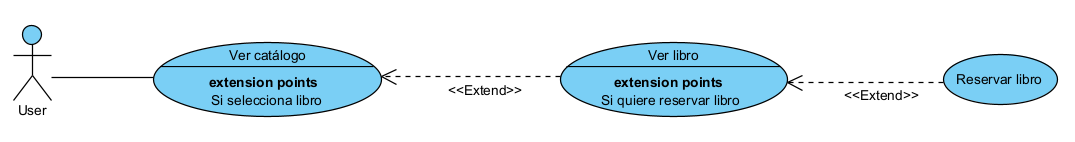
\includegraphics[width=0.8\textwidth]{./img/casos_uso/GestionDeReservas.png}
                            \\Figura 3.2.1.1: Diagrama de casos de uso de la subfuncionalidad de gestión de reservas
                        \end{figure}\\
                        \hline
                        \textbf{Nombre:} Ver libros recomendados\\
                        \hline
                        \textbf{Descripción:} Permite a los usuarios realizar reservas de libros.\\
                        \hline
                        \textbf{Actores:} Usuario\\
                        \hline
                        \textbf{Precondiciones:} Estar identificado en el sistema.\\
                        \hline
                        \textbf{Requisitos no funcionales:} Ninguno\\
                        \hline
                        \textbf{Flujo de Eventos:}
                        \begin{enumerate}
                            \item El usuario selecciona el libro deseado en el catálogo y pulsa “Reservar”. Se abre la interfaz de reserva (Figura 3.2.1.2).
                            \item Si el usuario pulsa aceptar, si el tiempo de reserva es menor a 2 meses aparece una interfaz indicando que la reserva se ha realizado con éxito (Figura 3.2.1.3).
                            \begin{enumerate}
                                \item Si el usuario pulsa aceptar, si el tiempo de reserva es mayor a 2 meses aparece una interfaz indicando error (Figura 3.2.1.4).
                                \item Si el usuario pulsa cancelar, se cierra la interfaz.
                            \end{enumerate}
                        \end{enumerate}\\
                        \hline
                        \textbf{Poscondiciones:} Ninguna\\
                        \hline
                        \textbf{Interfaz Gráfica:}\\
                        \begin{figure}[H]
                            \centering
                            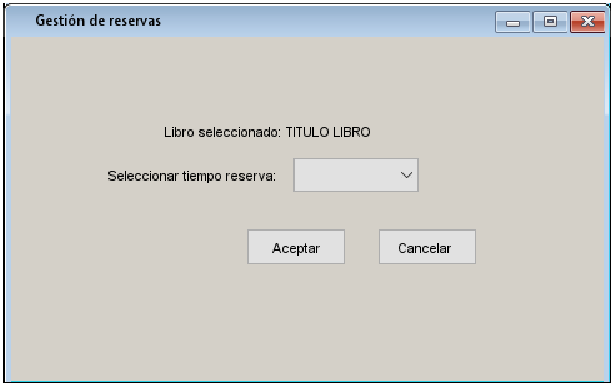
\includegraphics[width=0.8\textwidth]{./img/grafico/GestionDeReservas1.PNG}
                            \\Figura 3.2.1.2: Interfaz de reserva
                        \end{figure}\\
                        \begin{figure}[H]
                            \centering
                            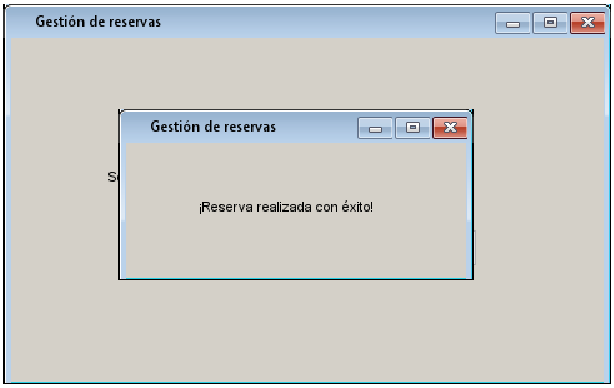
\includegraphics[width=0.8\textwidth]{./img/grafico/GestionDeReservas2.PNG}
                            \\Figura 3.2.1.3: Interfaz de reserva con éxito
                        \end{figure}\\
                        \begin{figure}[H]
                            \centering
                            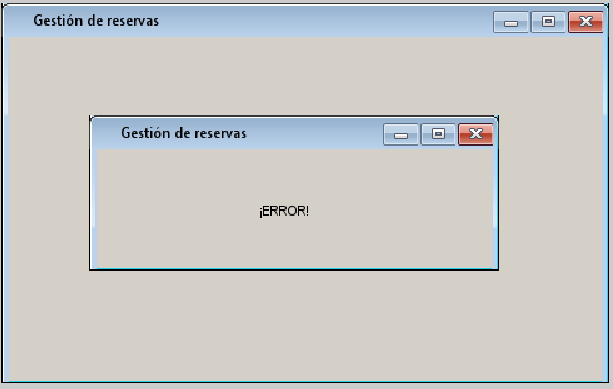
\includegraphics[width=0.8\textwidth]{./img/grafico/GestionDeReservas3.PNG}
                            \\Figura 3.2.1.4: Interfaz de reserva con error
                        \end{figure}\\
                        \hline
                    \end{longtable}
                \end{center}
            \clearpage
            \subsection{Reseñas}
                \begin{center}
                    \begin{longtable}{|p{\linewidth}|}
                        \hline
                        \textbf{Responsable:} Javier Criado\\
                        \hline
                        \begin{figure}[H]
                            \centering
                            \includegraphics[width=0.8\textwidth]{./img/casos_uso/Reseñas.png}
                            \\Figura 3.2.2.1: Diagrama de casos de uso de la subfuncionalidad de reseñas
                        \end{figure}\\
                        \hline
                        \textbf{Nombre:} Reseñas\\
                        \hline
                        \textbf{Descripción:} Permite al cliente puntuar y comentar en un libro una vez lo haya devuelto, también permite modificar estos datos posteriormente.\\
                        \hline
                        \textbf{Actores:} Usuario\\
                        \hline
                        \textbf{Precondiciones:} Estar identificado en el sistema\\
                        \hline
                        \textbf{Requisitos no funcionales:} Ninguno\\
                        \hline
                        \textbf{Flujo de Eventos:}
                        \begin{enumerate}
                            \item El usuario entra en el catalogo para ver los libros disponibles.
                            \begin{enumerate}
                                \item El usuario selecciona uno de los libros. [Figura 3.2.2.2]
                                \begin{enumerate}
                                    \item Al seleccionar 'Devolver libro', se devolvera el libro y se podra añadir una nueva reseña.
                                    \item Al seleccionar 'Escribir reseña', se abrira una pestaña donde se podrá escribir una reseña sobre el libro. [Figura 3.2.2.3]
                                    \item Al seleccionar el boton 'Ver reseñas', el usuario podrá ver las reseñas sobre el libro. [Figura 3.2.2.4]
                                    \begin{enumerate}
                                        \item Al hacer click sobre una de las reseñas esta se mostrara en una ventana aparte. [Figura 3.2.2.5]
                                    \end{enumerate}
                                \end{enumerate} 
                            \end{enumerate} 
                        \end{enumerate}\\
                        \hline
                        \textbf{Poscondiciones:} Ninguna\\
                        \hline
                        \textbf{Interfaz Gráfica:}\\
                        \begin{figure}[H]
                            \centering
                            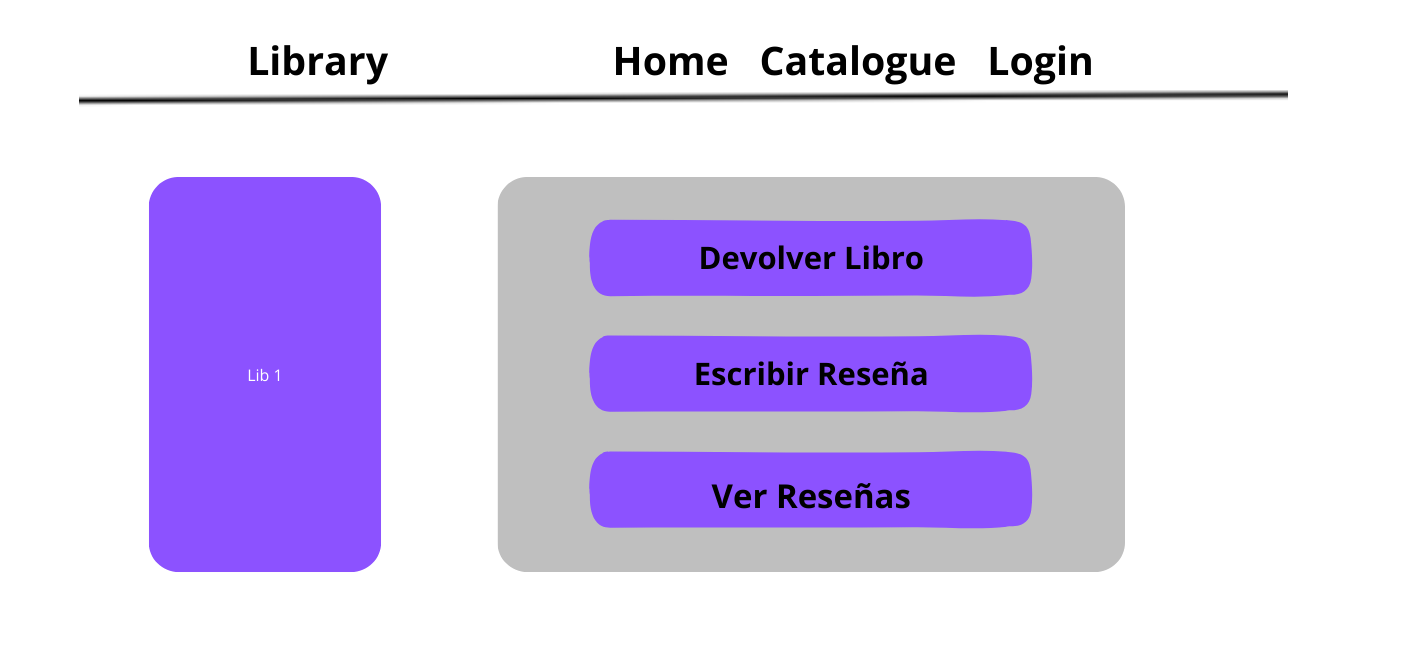
\includegraphics[width=0.8\textwidth]{./img/grafico/Ver_Libro.png}
                            \\Figura 3.2.2.2: Interfaz de ver libro.
                        \end{figure}\\
                        \begin{figure}[H]
                            \centering
                            \includegraphics[width=0.8\textwidth]{./img/grafico/Escribir_Reseña.png}
                            \\Figura 3.2.2.3: Interfaz de escribir reseña.
                        \end{figure}\\
                        \begin{figure}[H]
                            \centering
                            \includegraphics[width=0.8\textwidth]{./img/grafico/Ver_Reseñas.jpg}
                            \\Figura 3.2.2.4: Interfaz para ver las reseñas.
                        \end{figure}\\
                        \begin{figure}[H]
                            \centering
                            \includegraphics[width=0.8\textwidth]{./img/grafico/Ver_Una_Reseña.jpg}
                            \\Figura 3.2.2.5: Interfaz para ver una reseña.
                        \end{figure}\\
                        \hline
                    \end{longtable}
                \end{center}
                \clearpage
            \subsection{Red de amigos}
                \begin{center}
                    \begin{longtable}{|p{\linewidth}|}
                        \hline
                        \textbf{Responsable:} Jon Valdes\\
                        \hline
                        \begin{figure}[H]
                            \centering
                            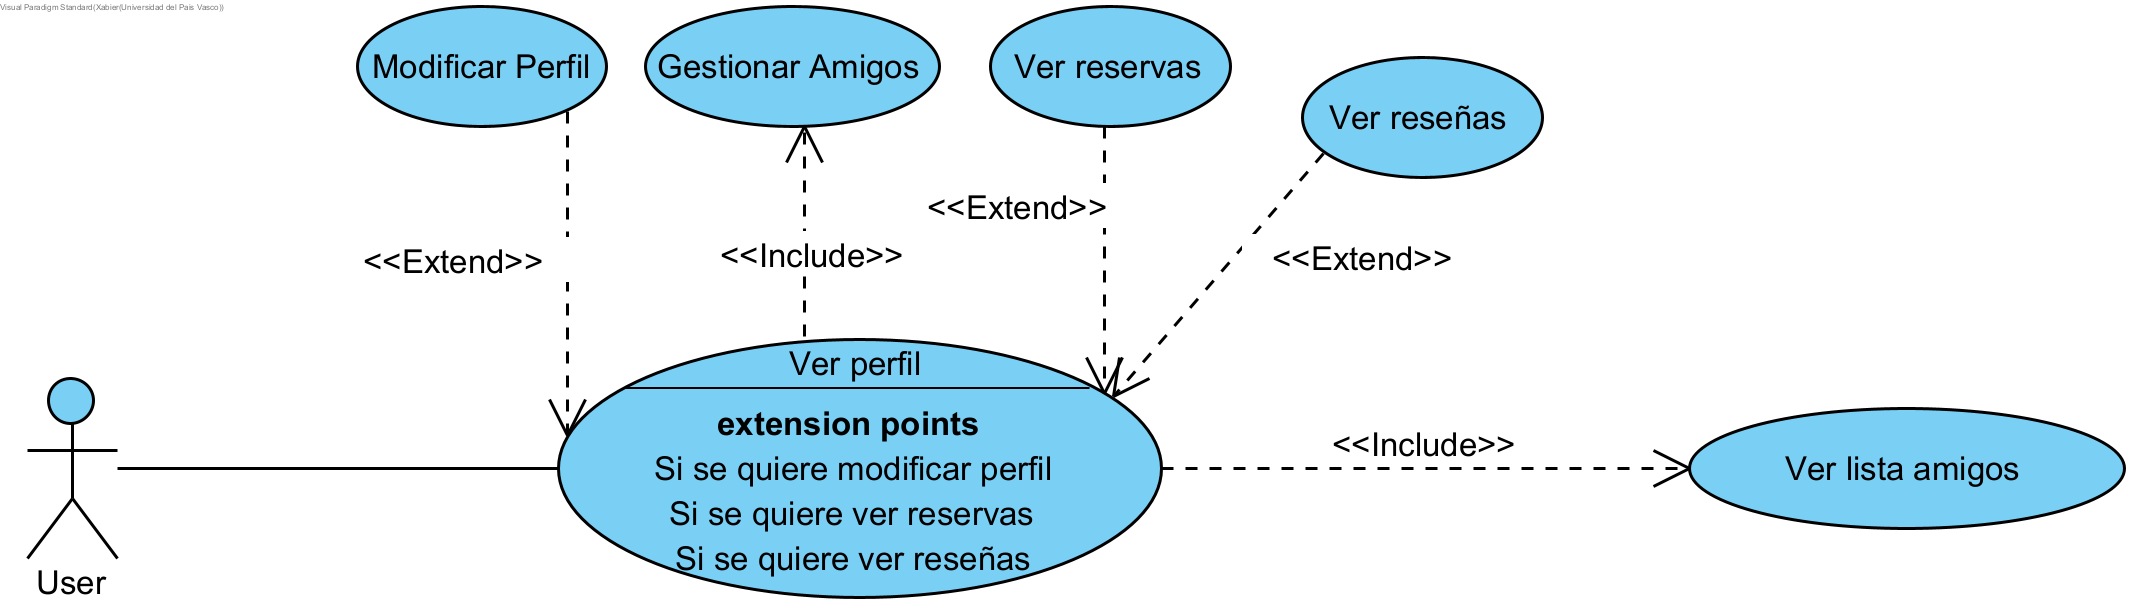
\includegraphics[width=0.8\textwidth]{./img/casos_uso/RedAmigos.png}
                            \\Figura 3.2.3.1: Diagrama de casos de uso de la subfuncionalidad de red de amigos
                        \end{figure}\\
                        \hline
                        \textbf{Nombre:} Red de amigos.\\
                        \hline
                        \textbf{Descripción:} Permite al usuario gestionar su perfil, de modo que puede tanto consultar el historial de reservas y de reseñas, como añadir o eliminar amigos. También puede editar sus datos personales.\\
                        \hline
                        \textbf{Actores:} Usuario.\\
                        \hline
                        \textbf{Precondiciones:} Estar identificado en el sistema.\\
                        \hline
                        \textbf{Requisitos no funcionales:} Ninguno\\
                        \hline
                        \textbf{Flujo de Eventos:}
                        \begin{enumerate}
                            \item El usuario accede a su perfil. [Figura 3.2.3.2]
                            \begin{enumerate}
                                \item El usuario puede pulsar 'Editar perfil' para editar sus datos. [Figura 3.2.3.5]
                                \item El usuario puede pulsar 'Consultar reservas' para ver su historial de reservas.
                                \item El usuario puede pulsar 'Consultar reseñas' para ver su historial de reseñas.
                                \item El usuario puede ver su lista de amigos.
                                \item El usuario puede pulsar 'Añadir amigo' para añadir un amigo. [Figura 3.2.3.3]
                                \item El usuario puede pulsar 'Solicutudes de amistad' para ver las solicitudes de amistad pendientes.
                                \item El usuario puede pulsar 'Eliminar amigo' para eliminar un amigo. [Figura 3.2.3.4]
                            \end{enumerate}
                        \end{enumerate}\\
                        \hline
                        \textbf{Poscondiciones:} Ninguna\\
                        \hline
                        \textbf{Interfaz Gráfica:}\\
                        \begin{figure}[H]
                            \centering
                            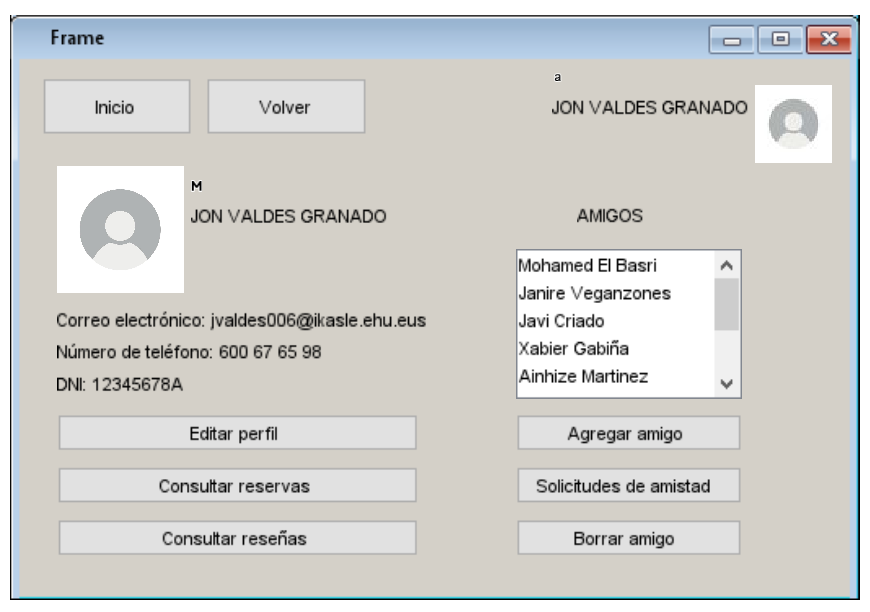
\includegraphics[width=0.8\textwidth]{./img/grafico/InterfazMenu.png}
                            \\Figura 3.2.3.2: Interfaz del perfil de usuario.
                        \end{figure}\\
                        \begin{figure}[H]
                            \centering
                            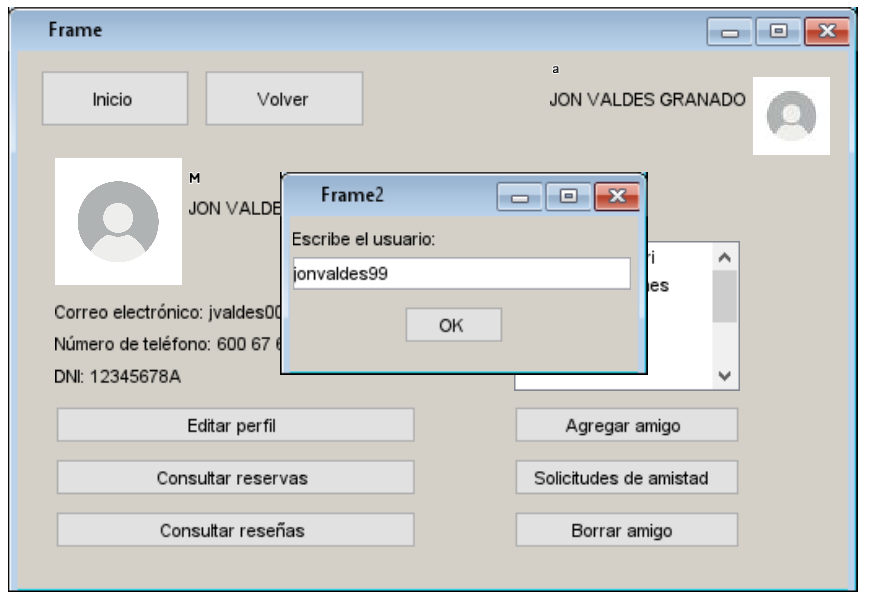
\includegraphics[width=0.8\textwidth]{./img/grafico/InterfazAnadrAmigo.png}
                            \\Figura 3.2.3.3: Interfaz para añadir un amigo.
                        \end{figure}\\
                        \begin{figure}[H]
                            \centering
                            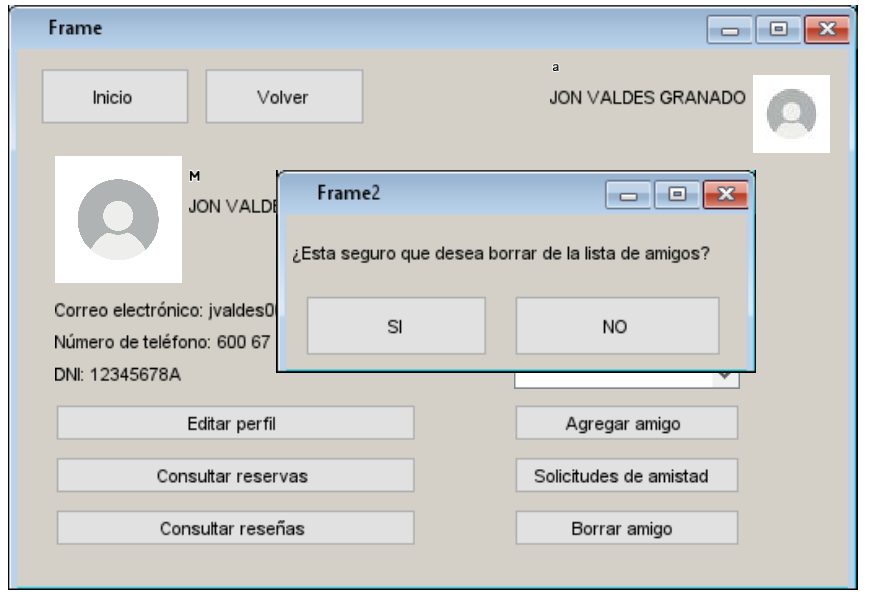
\includegraphics[width=0.8\textwidth]{./img/grafico/interfazAlertaBorrarAmigo.png}
                            \\Figura 3.2.3.4: Interfaz de alerta para borrar un amigo.
                        \end{figure}\\
                        \begin{figure}[H]
                            \centering
                            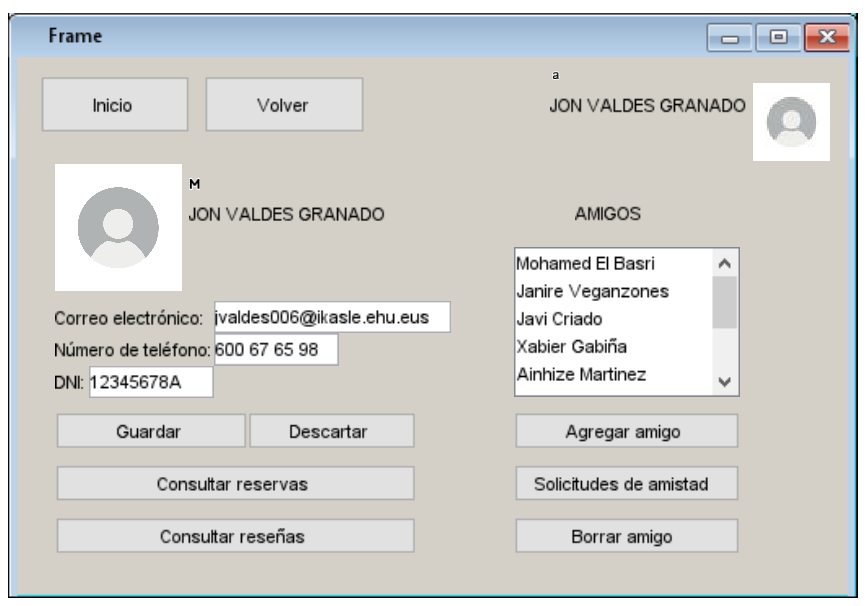
\includegraphics[width=0.8\textwidth]{./img/grafico/InterfazEditarPerfil.png}
                            \\Figura 3.2.3.5: Interfaz para editar el perfil.
                        \end{figure}\\
                        \hline
                    \end{longtable}
                \end{center}
                \clearpage
            \subsection{Administrador}
                \subsubsection*{Gestión de usuarios}
                    \begin{center}
                        \begin{longtable}{|p{\linewidth}|}
                            \hline
                            \textbf{Responsable:} Janire Veganzones\\
                            \hline
                            \begin{figure}[H]
                                \centering
                                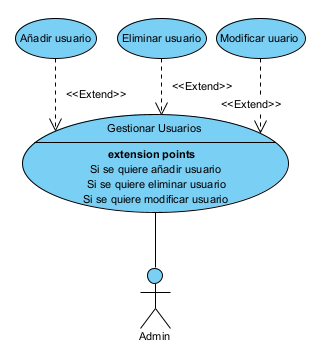
\includegraphics[width=0.45\textwidth]{./img/casos_uso/GestionarUsuarios.png}
                                \\Figura 3.2.4.1.1: Diagrama de casos de uso de la subfuncionalidad de gestión de usuarios
                            \end{figure}\\
                            \hline
                            \textbf{Nombre:} Gestionar usuarios\\
                            \hline
                            \textbf{Descripción:}  Permite crear, eliminar o modificar un usuario en el sistema.\\
                            \hline
                            \textbf{Actores:} Admin\\
                            \hline
                            \textbf{Precondiciones:} Estar identificado en el sistema y ser administrador.\\
                            \hline
                            \textbf{Requisitos no funcionales:} Ninguno\\
                            \hline
                            \textbf{Flujo de Eventos:}
                            \begin{enumerate}
                                \item Se accede al menu de administrador. [Figura 3.2.4.1.2]
                                \begin{enumerate}
                                    \item Se selecciona la opción de gestionar usuarios. [Figura 3.2.4.1.3]
                                    \begin{enumerate}
                                        \item El administrador pulsa 'Crear' para crear un nuevo usuario. [Figura 3.2.4.1.4]
                                        \begin{enumerate}
                                            \item Si hay un error al crear un usuario saldra un error mostrandolo. [Figura 3.2.4.1.5]
                                        \end{enumerate}
                                        \item El administrador pulsa 'Borrar' para borrar un usuario. [Figura 3.2.4.1.6]
                                        \begin{enumerate}
                                            \item Si el usuario a borrar no existe mostrara un error. [Figura 3.2.4.1.7]
                                        \end{enumerate}
                                        \item El administrador pulsa 'Modificar' para modificar un usuario. [Figura 3.2.4.1.8]
                                        \begin{enumerate}
                                            \item Si hay un error al modificar un usuario saldra un error mostrandolo. [Figura 3.2.4.1.9]
                                        \end{enumerate}
                                    \end{enumerate}
                                \end{enumerate} 
                            \end{enumerate}\\
                            \hline
                            \textbf{Poscondiciones:} Ninguna\\
                            \hline
                            \textbf{Interfaz Gráfica:}\\
                            \begin{figure}[H]
                                \centering
                                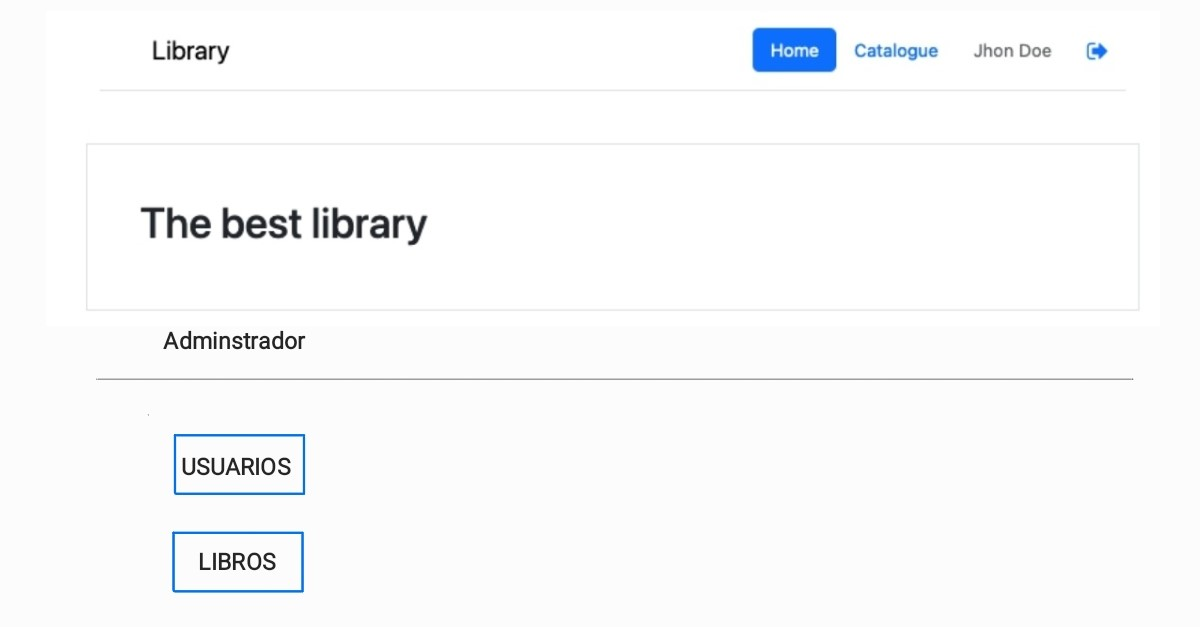
\includegraphics[width=0.8\textwidth]{./img/grafico/MenuAdmin.jpg}
                                \\Figura 3.2.4.1.2: Interfaz del menú de administrador.
                            \end{figure}\\
                            \begin{figure}[H]
                                \centering
                                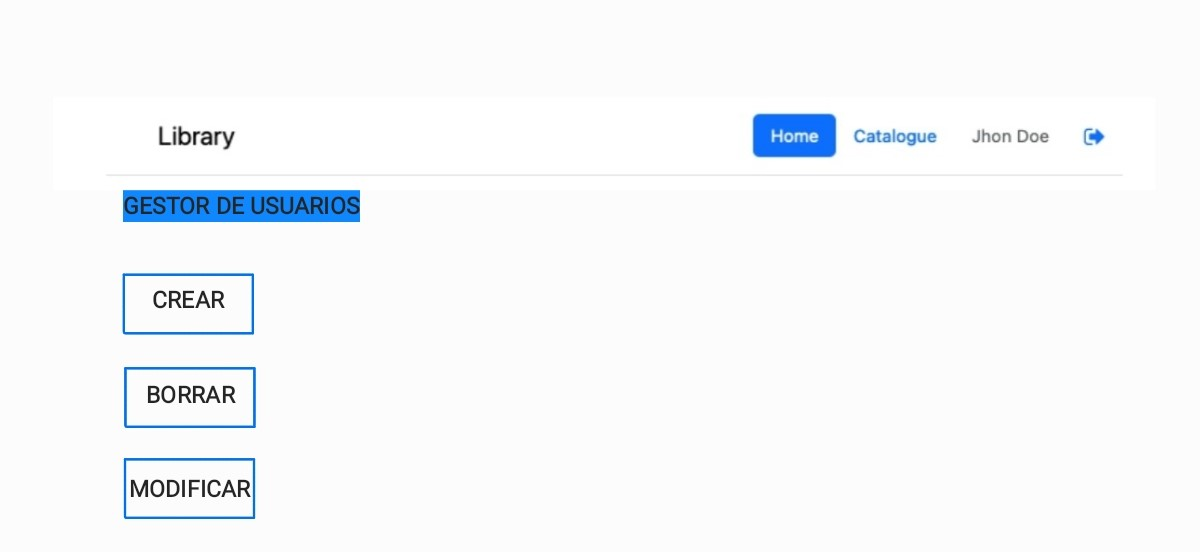
\includegraphics[width=0.8\textwidth]{./img/grafico/MenuGestorUsu.jpg}
                                \\Figura 3.2.4.1.3: Interfaz del menu de gestión de usuarios.
                            \end{figure}\\
                            \begin{figure}[H]
                                \centering
                                \includegraphics[width=0.8\textwidth]{./img/grafico/AñadirUsu.jpg}
                                \\Figura 3.2.4.1.4: Interfaz para añadir un usuario.
                            \end{figure}\\
                            \begin{figure}[H]
                                \centering
                                \includegraphics[width=0.8\textwidth]{./img/grafico/ErrorAñadirUsu.jpg}
                                \\Figura 3.2.4.1.5: Interfaz de error al añadir un usuario.
                            \end{figure}\\
                            \begin{figure}[H]
                                \centering
                                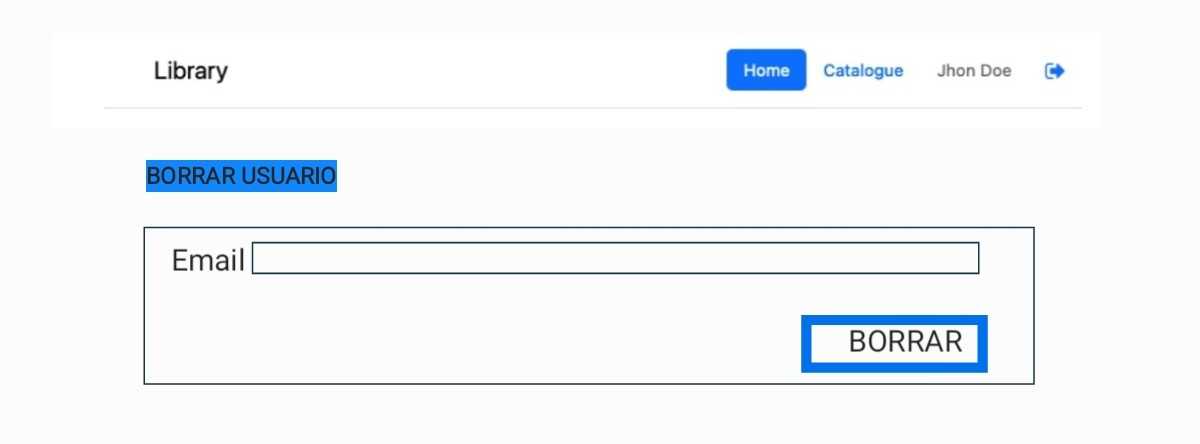
\includegraphics[width=0.8\textwidth]{./img/grafico/BorrarUsu.jpg}
                                \\Figura 3.2.4.1.6: Interfaz para borrar un usuario.
                            \end{figure}\\
                            \begin{figure}[H]
                                \centering
                                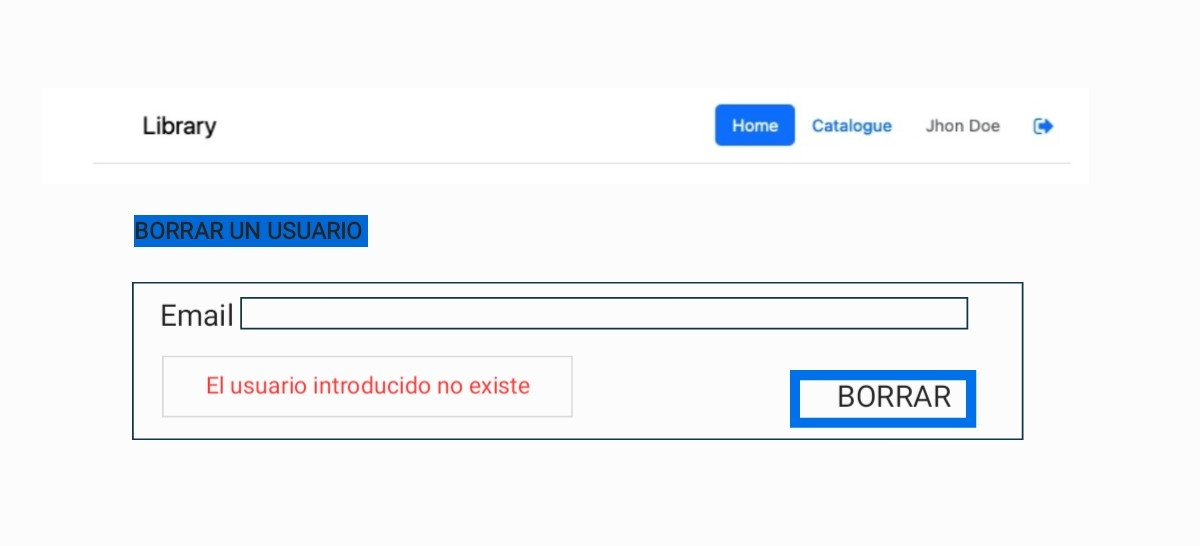
\includegraphics[width=0.8\textwidth]{./img/grafico/ErrorBorrarUsu.jpg}
                                \\Figura 3.2.4.1.7: Interfaz de error al borrar un usuario.
                            \end{figure}\\
                            \begin{figure}[H]
                                \centering
                                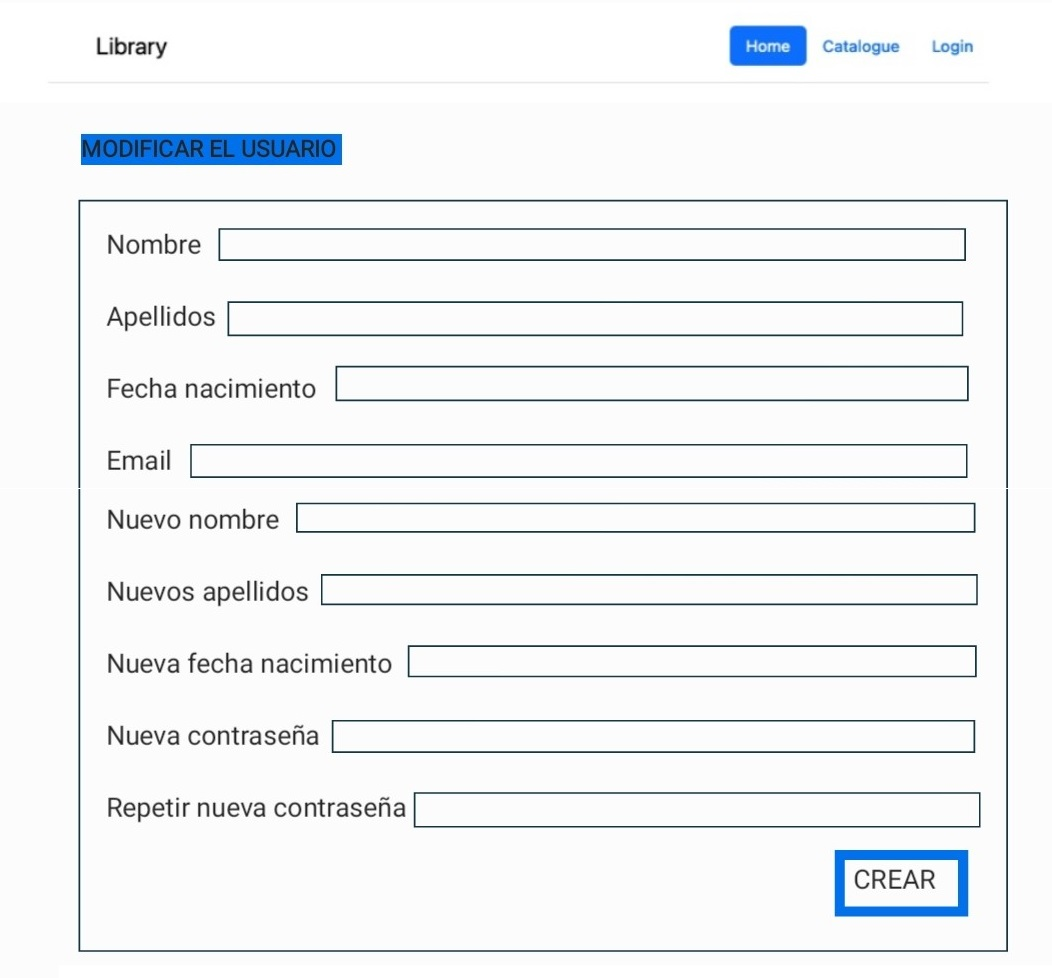
\includegraphics[width=0.8\textwidth]{./img/grafico/ModificarUsu.jpg}
                                \\Figura 3.2.4.1.8: Interfaz para modificar un usuario.
                            \end{figure}\\
                            \begin{figure}[H]
                                \centering
                                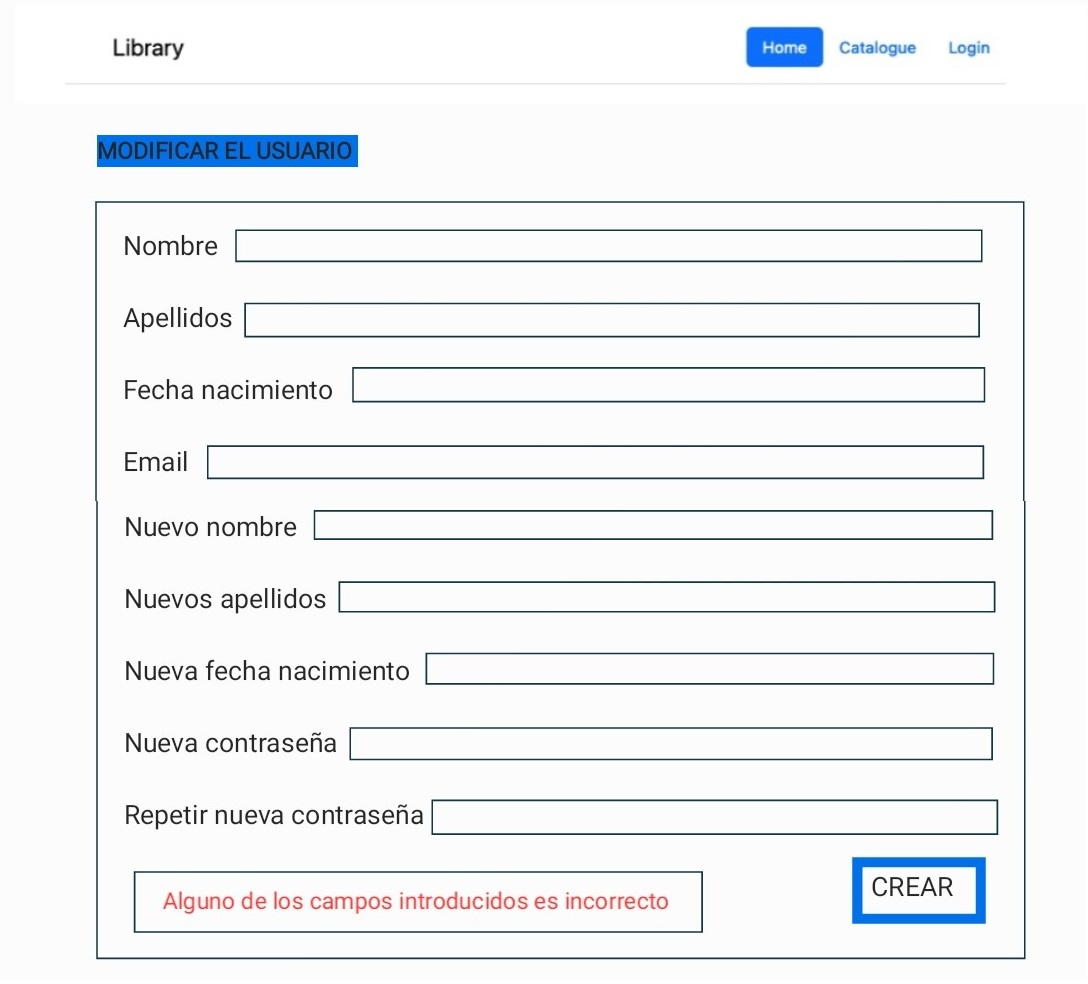
\includegraphics[width=0.8\textwidth]{./img/grafico/ErrorModificarUsu.jpg}
                                \\Figura 3.2.4.1.9: Interfaz de error al modificar un usuario.
                            \end{figure}\\
                            \hline
                        \end{longtable}
                    \end{center}
                    \clearpage
                \subsubsection*{Gestión de libros}
                    \begin{center}
                        \begin{longtable}{|p{\linewidth}|}
                            \hline
                            \textbf{Responsable:} Janire Veganzones\\
                            \hline
                            \begin{figure}[H]
                                \centering
                                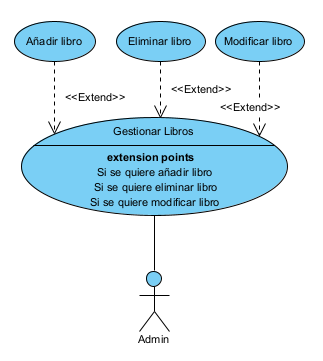
\includegraphics[width=0.45\textwidth]{./img/casos_uso/GestionarLibros.png}
                                \\Figura 3.2.4.2.1: Diagrama de casos de uso de la subfuncionalidad de gestión de libros
                            \end{figure}\\
                            \hline
                            \textbf{Nombre:} Gestionar libros\\
                            \hline
                            \textbf{Descripción:}  Permite añadir, eliminar o modificar un libro en el sistema.\\
                            \hline
                            \textbf{Actores:} Admin\\
                            \hline
                            \textbf{Precondiciones:} Estar identificado en el sistema y ser usuario.\\
                            \hline
                            \textbf{Requisitos no funcionales:} Ninguno\\
                            \hline
                            \textbf{Flujo de Eventos:}
                            \begin{enumerate}
                                \item Se accede al menu de administrador. [Figura 3.2.4.2.2]
                                \begin{enumerate}
                                    \item Se selecciona la opción de gestionar libros. [Figura 3.2.4.2.3]
                                    \begin{enumerate}
                                        \item El administrador pulsa 'Crear' para crear un nuevo libro. [Figura 3.2.4.2.4]
                                        \begin{enumerate}
                                            \item Si hay un error al crear un libro saldra un error mostrandolo. [Figura 3.2.4.2.5]
                                        \end{enumerate}
                                        \item El administrador pulsa 'Borrar' para borrar un libro. [Figura 3.2.4.2.6]
                                        \begin{enumerate}
                                            \item Si el libro a borrar no existe mostrara un error. [Figura 3.2.4.2.7]
                                        \end{enumerate}
                                        \item El administrador pulsa 'Modificar' para modificar un libro. [Figura 3.2.4.2.8]
                                        \begin{enumerate}
                                            \item Si hay un error al modificar un libro saldra un error mostrandolo. [Figura 3.2.4.2.9]
                                        \end{enumerate}
                                    \end{enumerate}
                                \end{enumerate} 
                            \end{enumerate}\\
                            \hline
                            \textbf{Poscondiciones:} Ninguna\\
                            \hline
                            \textbf{Interfaz Gráfica:}\\
                            \begin{figure}[H]
                                \centering
                                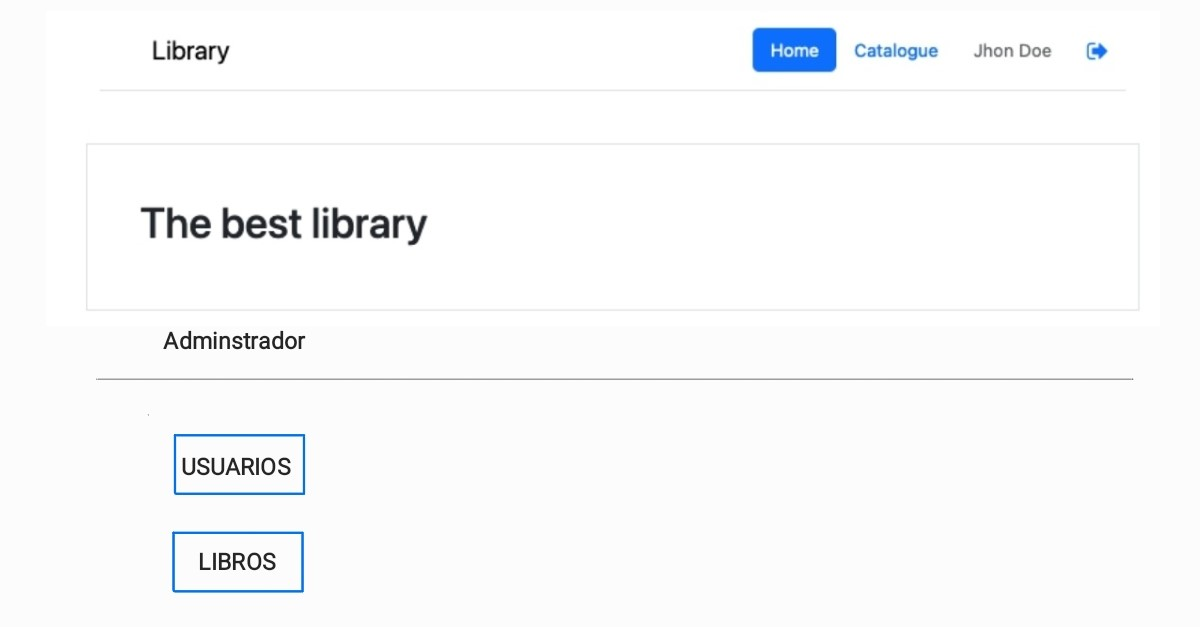
\includegraphics[width=0.8\textwidth]{./img/grafico/MenuAdmin.jpg}
                                \\Figura 3.2.4.2.2: Interfaz del menú de administrador.
                            \end{figure}\\
                            \begin{figure}[H]
                                \centering
                                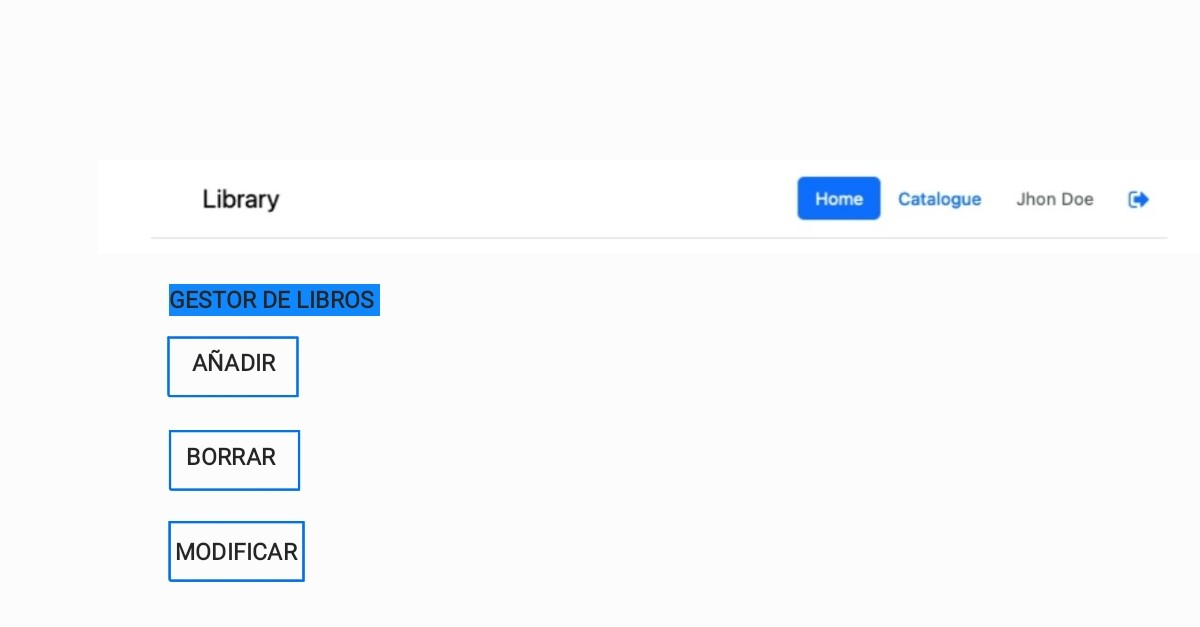
\includegraphics[width=0.8\textwidth]{./img/grafico/MenuGestorLibros.jpg}
                                \\Figura 3.2.4.2.3: Interfaz del menu de gestión de libros.
                            \end{figure}\\
                            \begin{figure}[H]
                                \centering
                                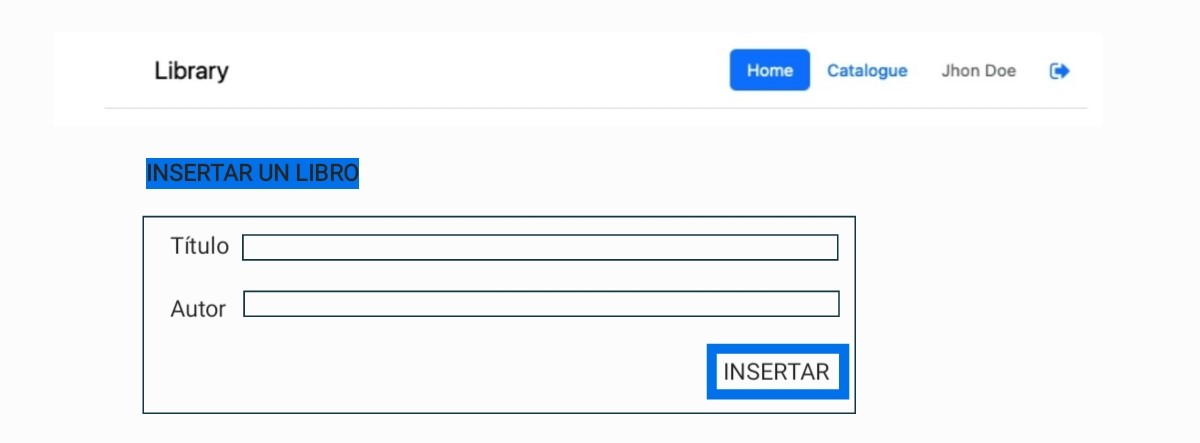
\includegraphics[width=0.8\textwidth]{./img/grafico/InsertarLibro.jpg}
                                \\Figura 3.2.4.2.4: Interfaz para añadir un libro.
                            \end{figure}\\
                            \begin{figure}[H]
                                \centering
                                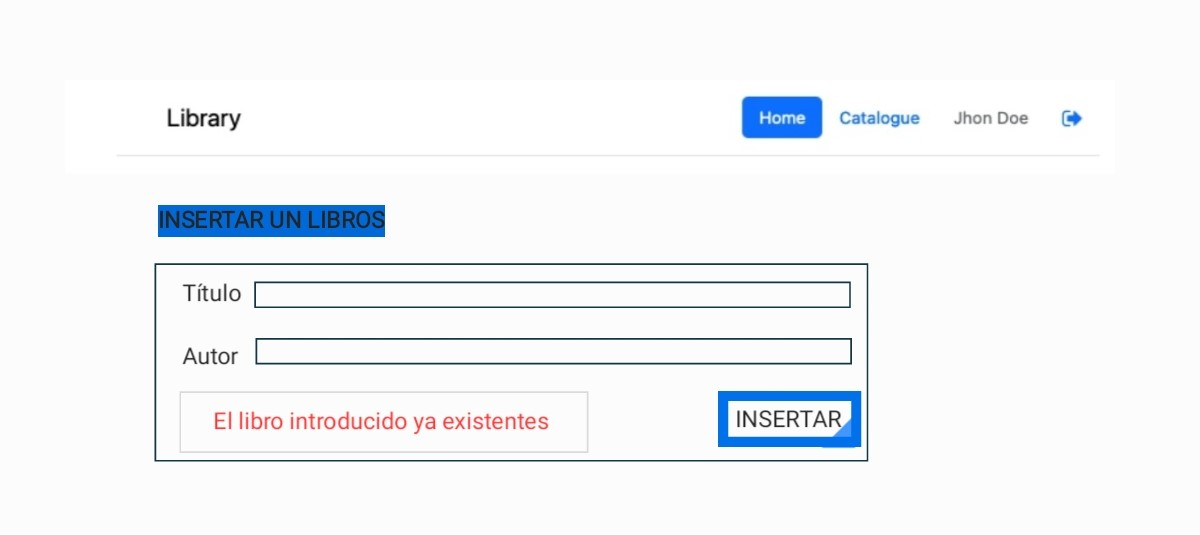
\includegraphics[width=0.8\textwidth]{./img/grafico/ErrorInsertarLibro.jpg}
                                \\Figura 3.2.4.2.5: Interfaz de error al añadir un libro.
                            \end{figure}\\
                            \begin{figure}[H]
                                \centering
                                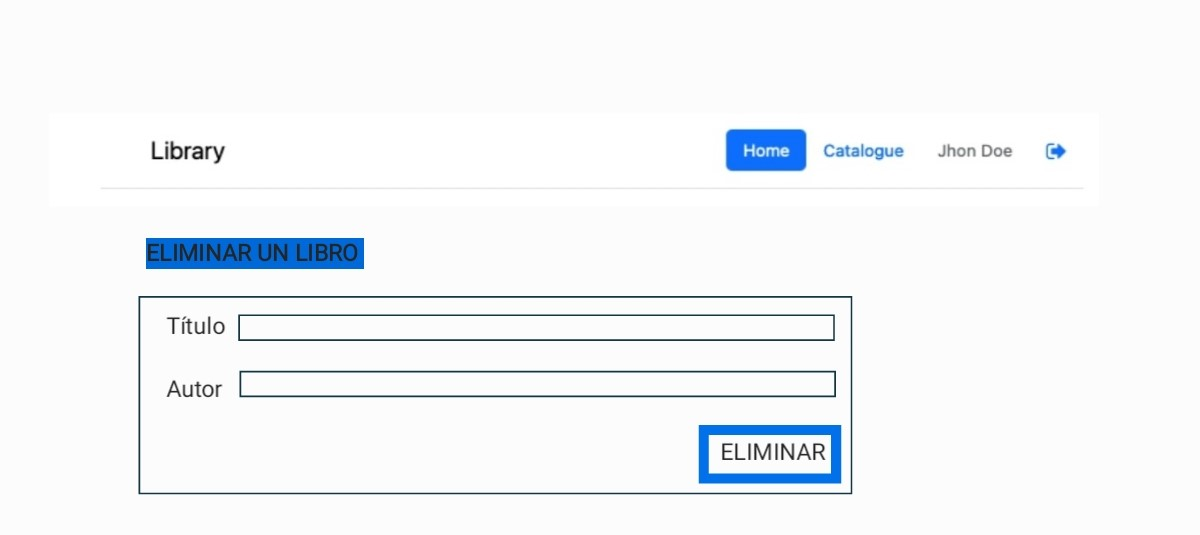
\includegraphics[width=0.8\textwidth]{./img/grafico/EliminarLibro.jpg}
                                \\Figura 3.2.4.2.6: Interfaz para borrar un libro.
                            \end{figure}\\
                            \begin{figure}[H]
                                \centering
                                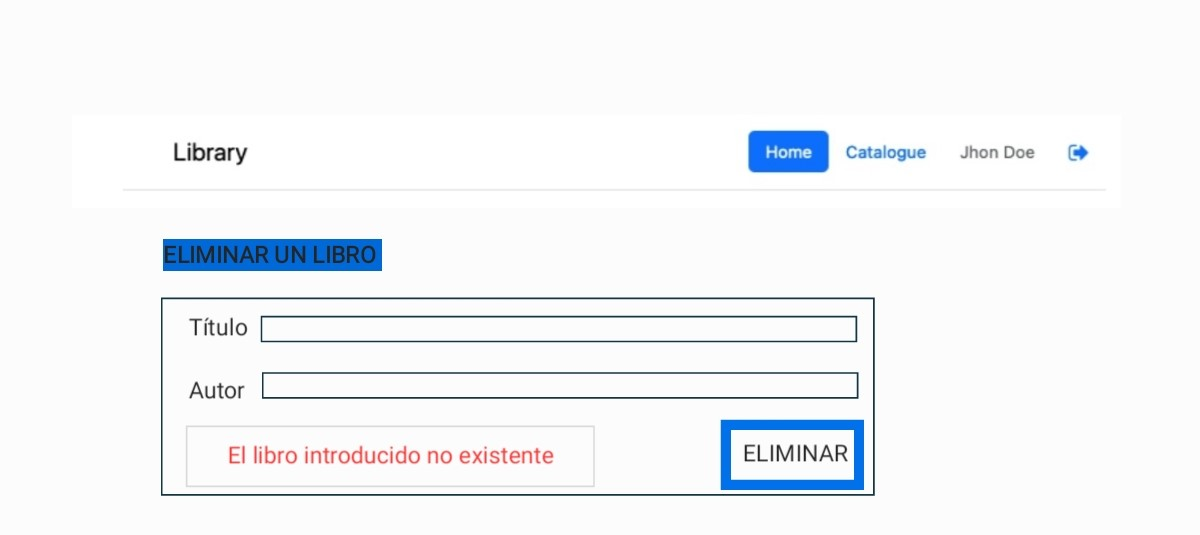
\includegraphics[width=0.8\textwidth]{./img/grafico/ErrorEliminarLibro.jpg}
                                \\Figura 3.2.4.2.7: Interfaz de error al borrar un libro.
                            \end{figure}\\
                            \begin{figure}[H]
                                \centering
                                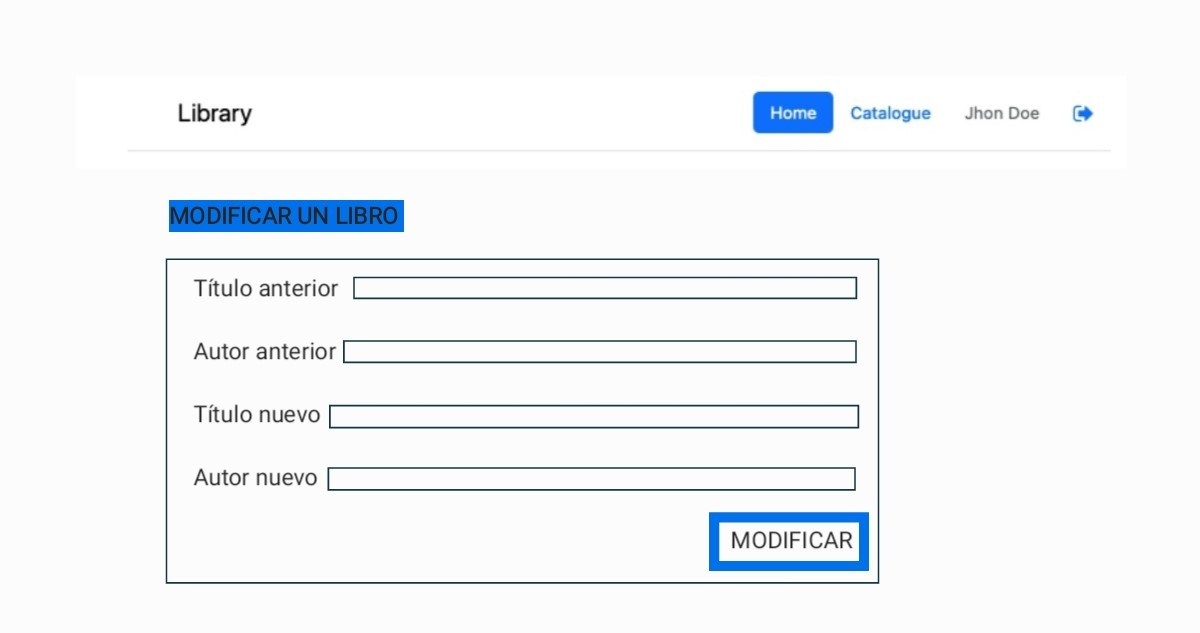
\includegraphics[width=0.8\textwidth]{./img/grafico/ModificarLibro.jpg}
                                \\Figura 3.2.4.2.8: Interfaz para modificar un libro.
                            \end{figure}\\
                            \begin{figure}[H]
                                \centering
                                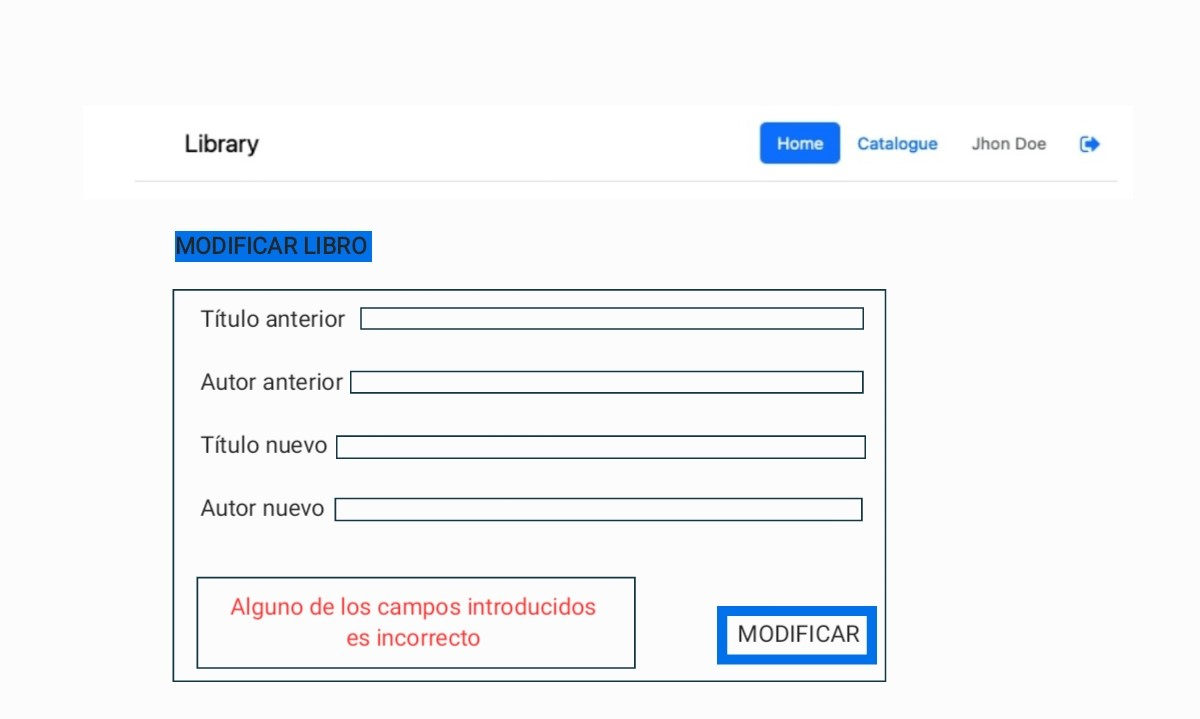
\includegraphics[width=0.8\textwidth]{./img/grafico/ErrorModificarLibro.jpg}
                                \\Figura 3.2.4.2.9: Interfaz de error al modificar un libro.
                            \end{figure}\\
                            \hline
                        \end{longtable}
                    \end{center}
                    \clearpage
            \subsection{Foros}
                \begin{center}
                    \begin{longtable}{|p{\linewidth}|}
                        \hline
                        \textbf{Responsable:} Ainhize Martinez\\
                        \hline
                        \begin{figure}[H]
                            \centering
                            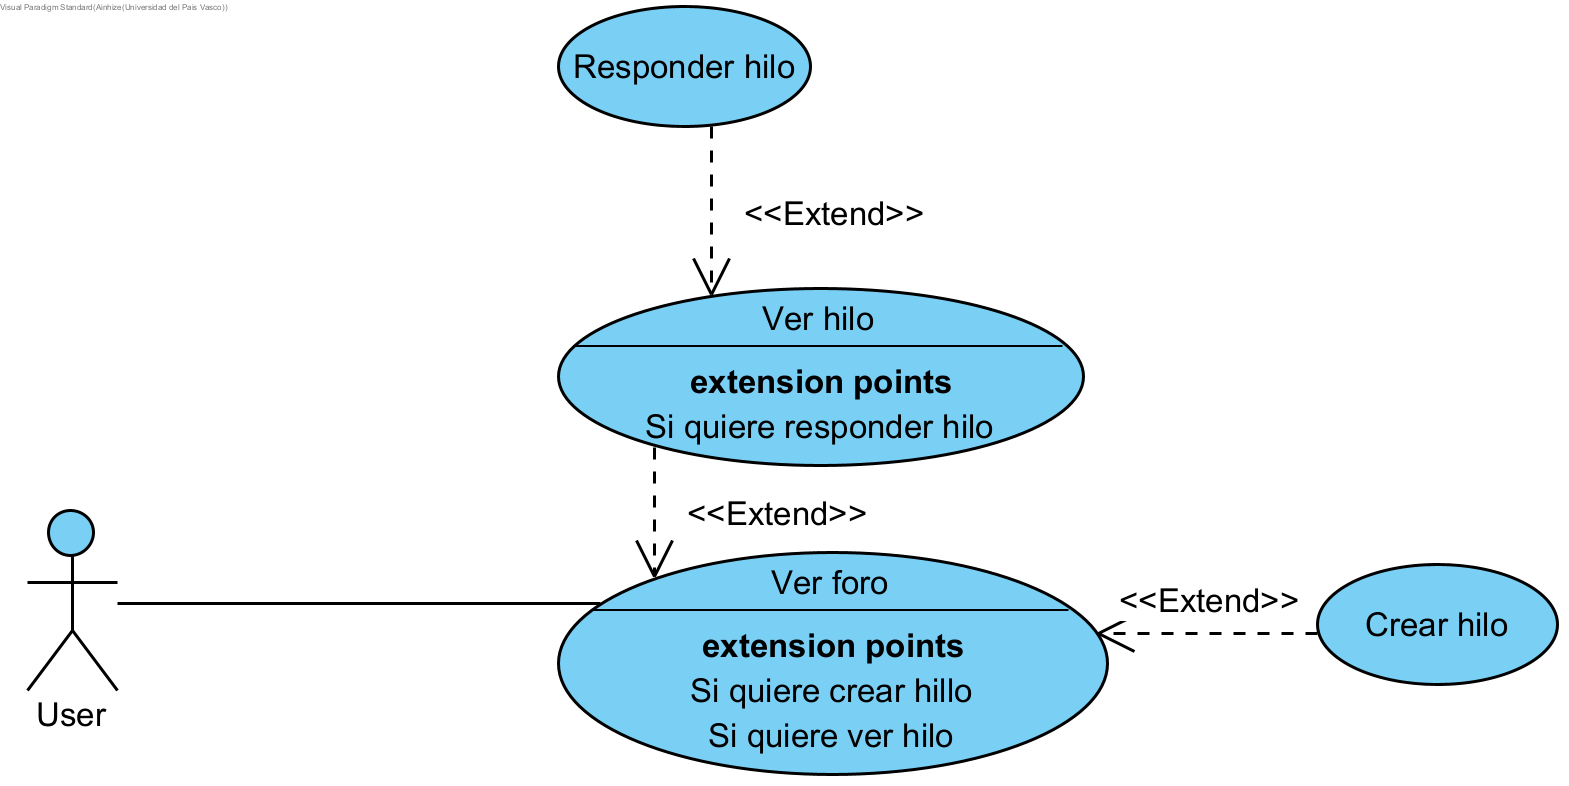
\includegraphics[width=0.8\textwidth]{./img/casos_uso/CasoForo.png}
                            \\Figura 3.2.5.1: Diagrama de casos de uso de la subfuncionalidad de foros
                        \end{figure}\\
                        \hline
                        \textbf{Nombre:} Ver Foros\\
                        \hline
                        \textbf{Descripción:} Permite al usuario acceder al foro, crear hilos nuevos, explorar todos los hilos, además de contestar hilos.\\
                        \hline
                        \textbf{Actores:} Usuario\\
                        \hline
                        \textbf{Precondiciones:} Estar identificado en el sistema.\\
                        \hline
                        \textbf{Requisitos no funcionales:} Ninguno\\
                        \hline
                        \textbf{Flujo de Eventos:}
                        \begin{enumerate}
                            \item El usuario selecciona 'Foro' para acceder a él.
                            \begin{enumerate}
                                \item Se le muestra toda la lista de hilos. [Figura 3.2.5.2]
                                \begin{enumerate}
                                    \item Si el usuario pulsa en '+Hilo' se le abre una ventana para crear un hilo nuevo. [Figura 3.2.5.3]
                                    \item Si el usuario selecciona un hilo se le mostraran las respuesta al hilo. [Figura 3.2.5.4]
                                    \begin{enumerate}
                                        \item Si el usuario pulsa en '+Mensaje' se le abre una ventana para responder al hilo [Figura 3.2.5.5]
                                    \end{enumerate}
                                \end{enumerate}
                            \end{enumerate}
                        \end{enumerate}\\
                        \hline
                        \textbf{Poscondiciones:} Ninguna\\
                        \hline
                        \textbf{Interfaz Gráfica:}\\
                        \begin{figure}[H]
                            \centering
                            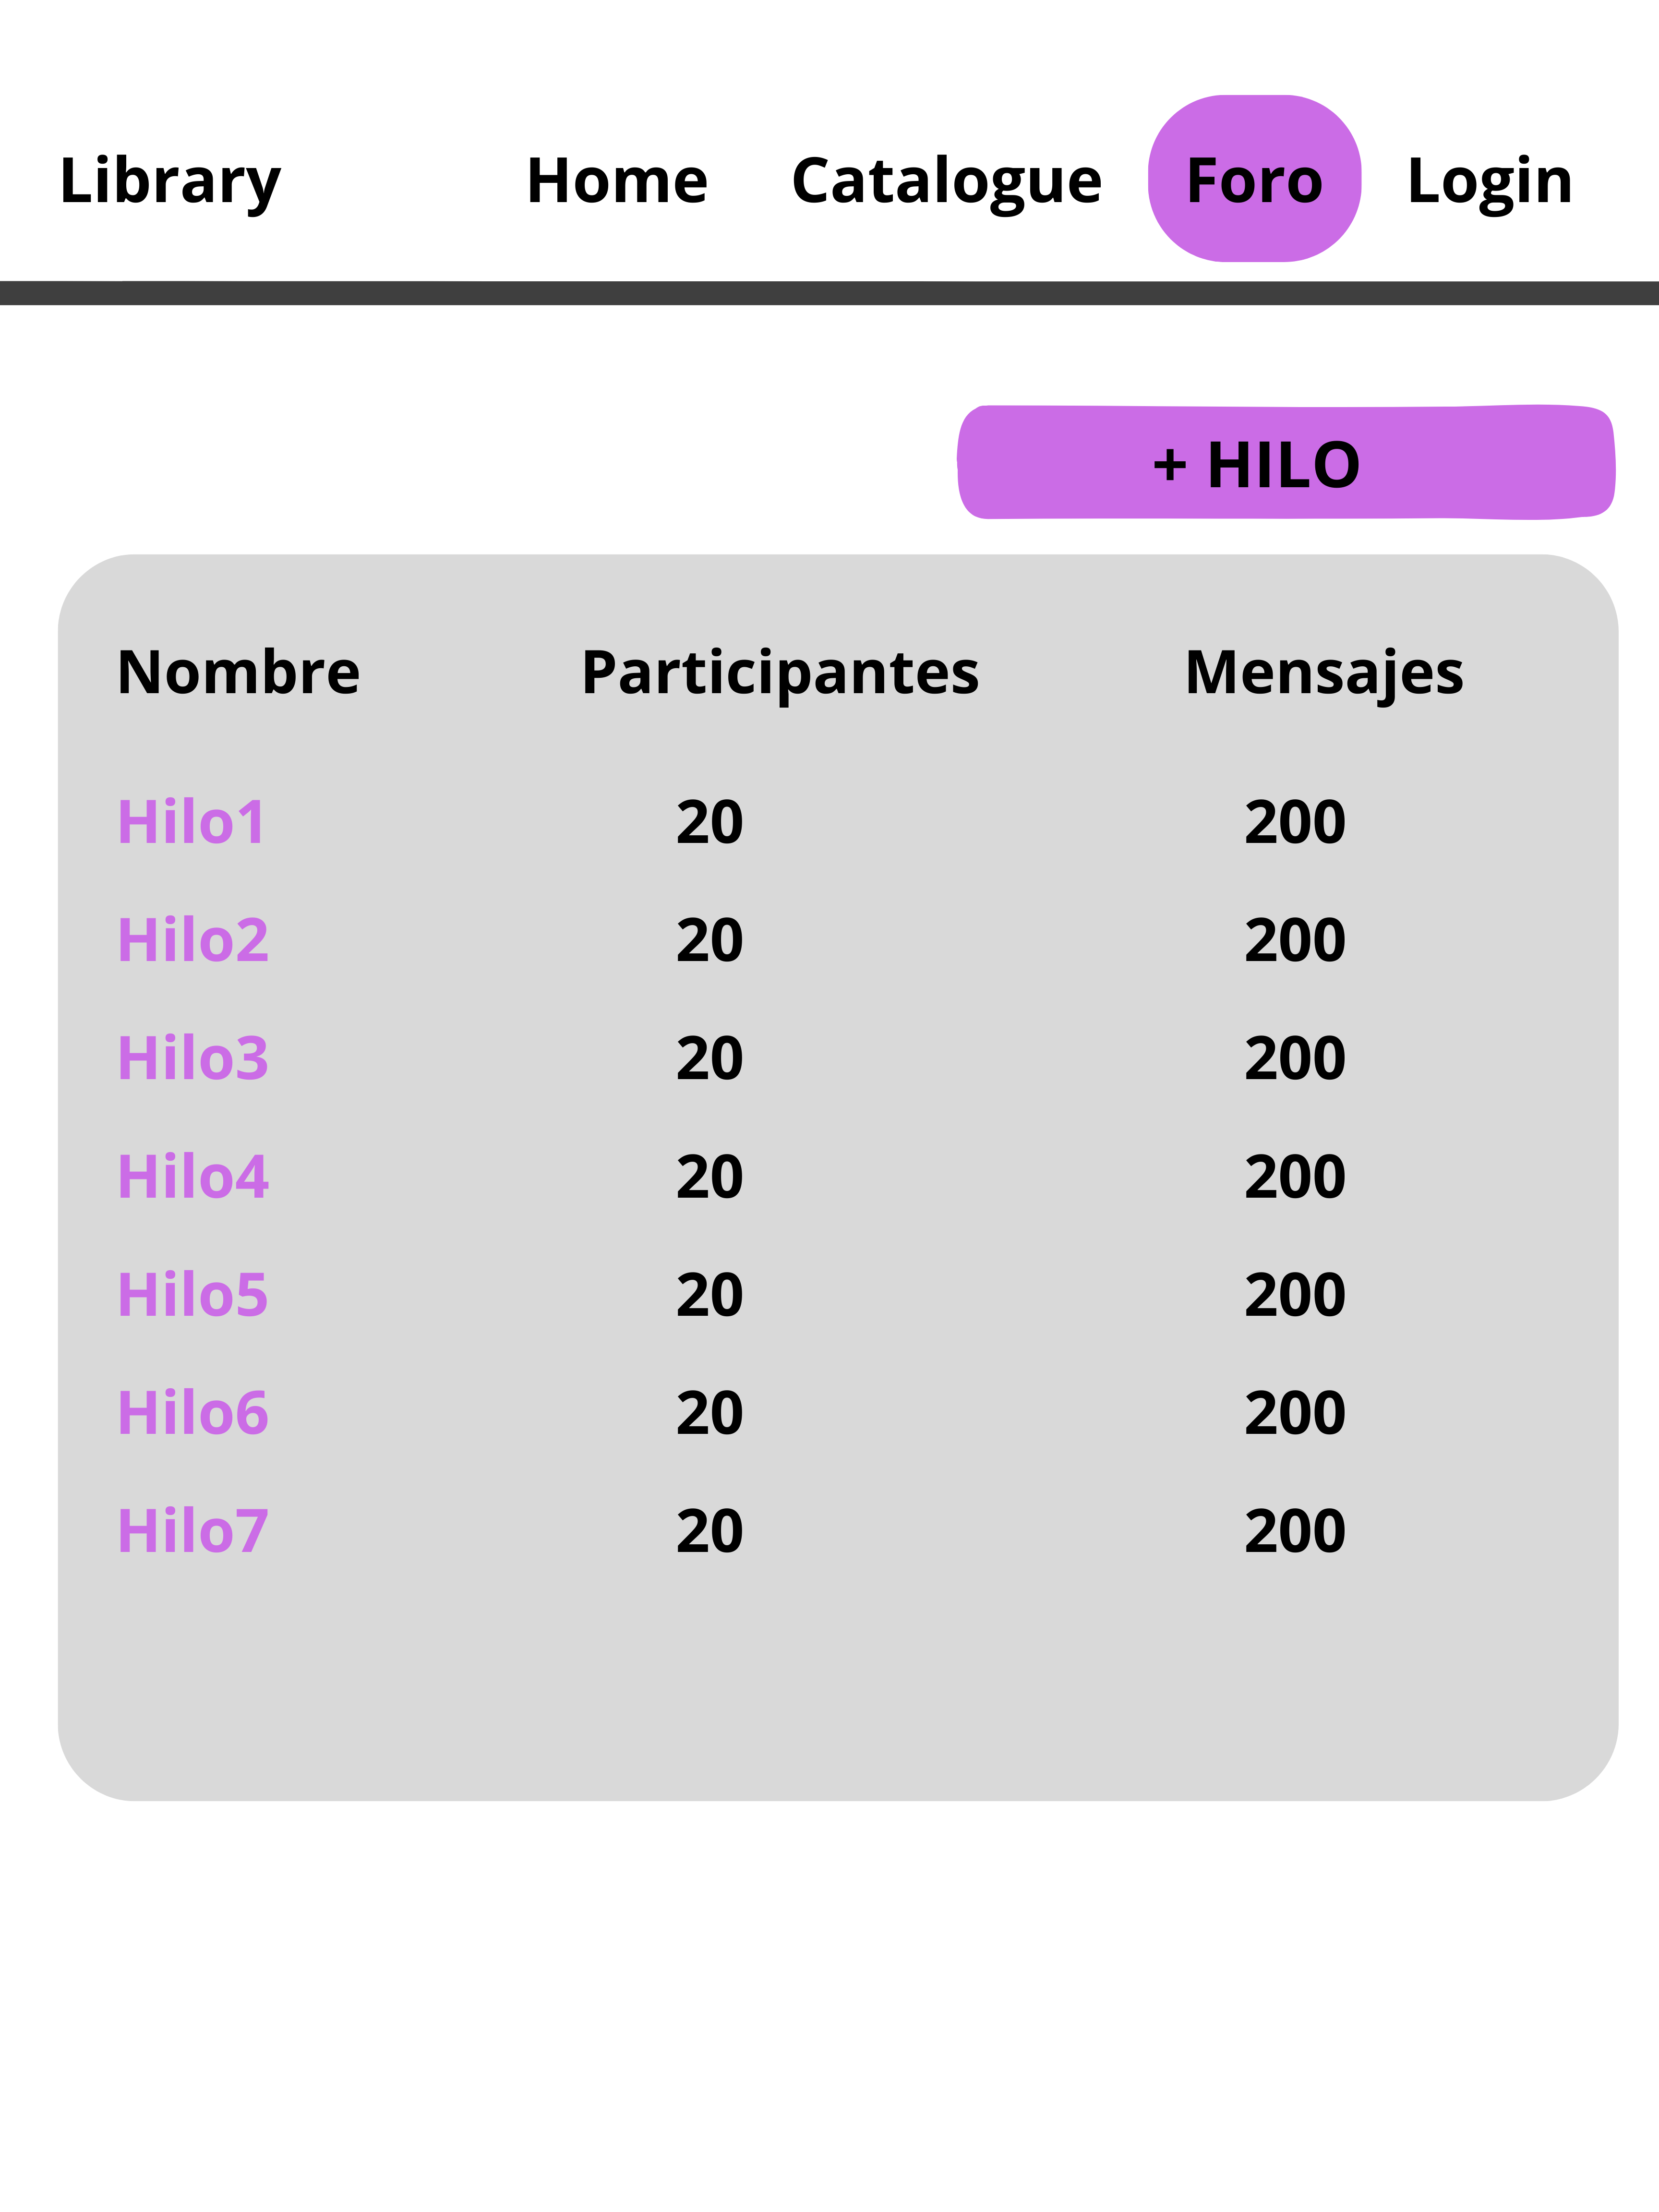
\includegraphics[width=0.8\textwidth]{./img/grafico/Foro.png}
                            \\Figura 3.2.5.2: Interfaz del foro.
                        \end{figure}\\
                        \begin{figure}[H]
                            \centering
                            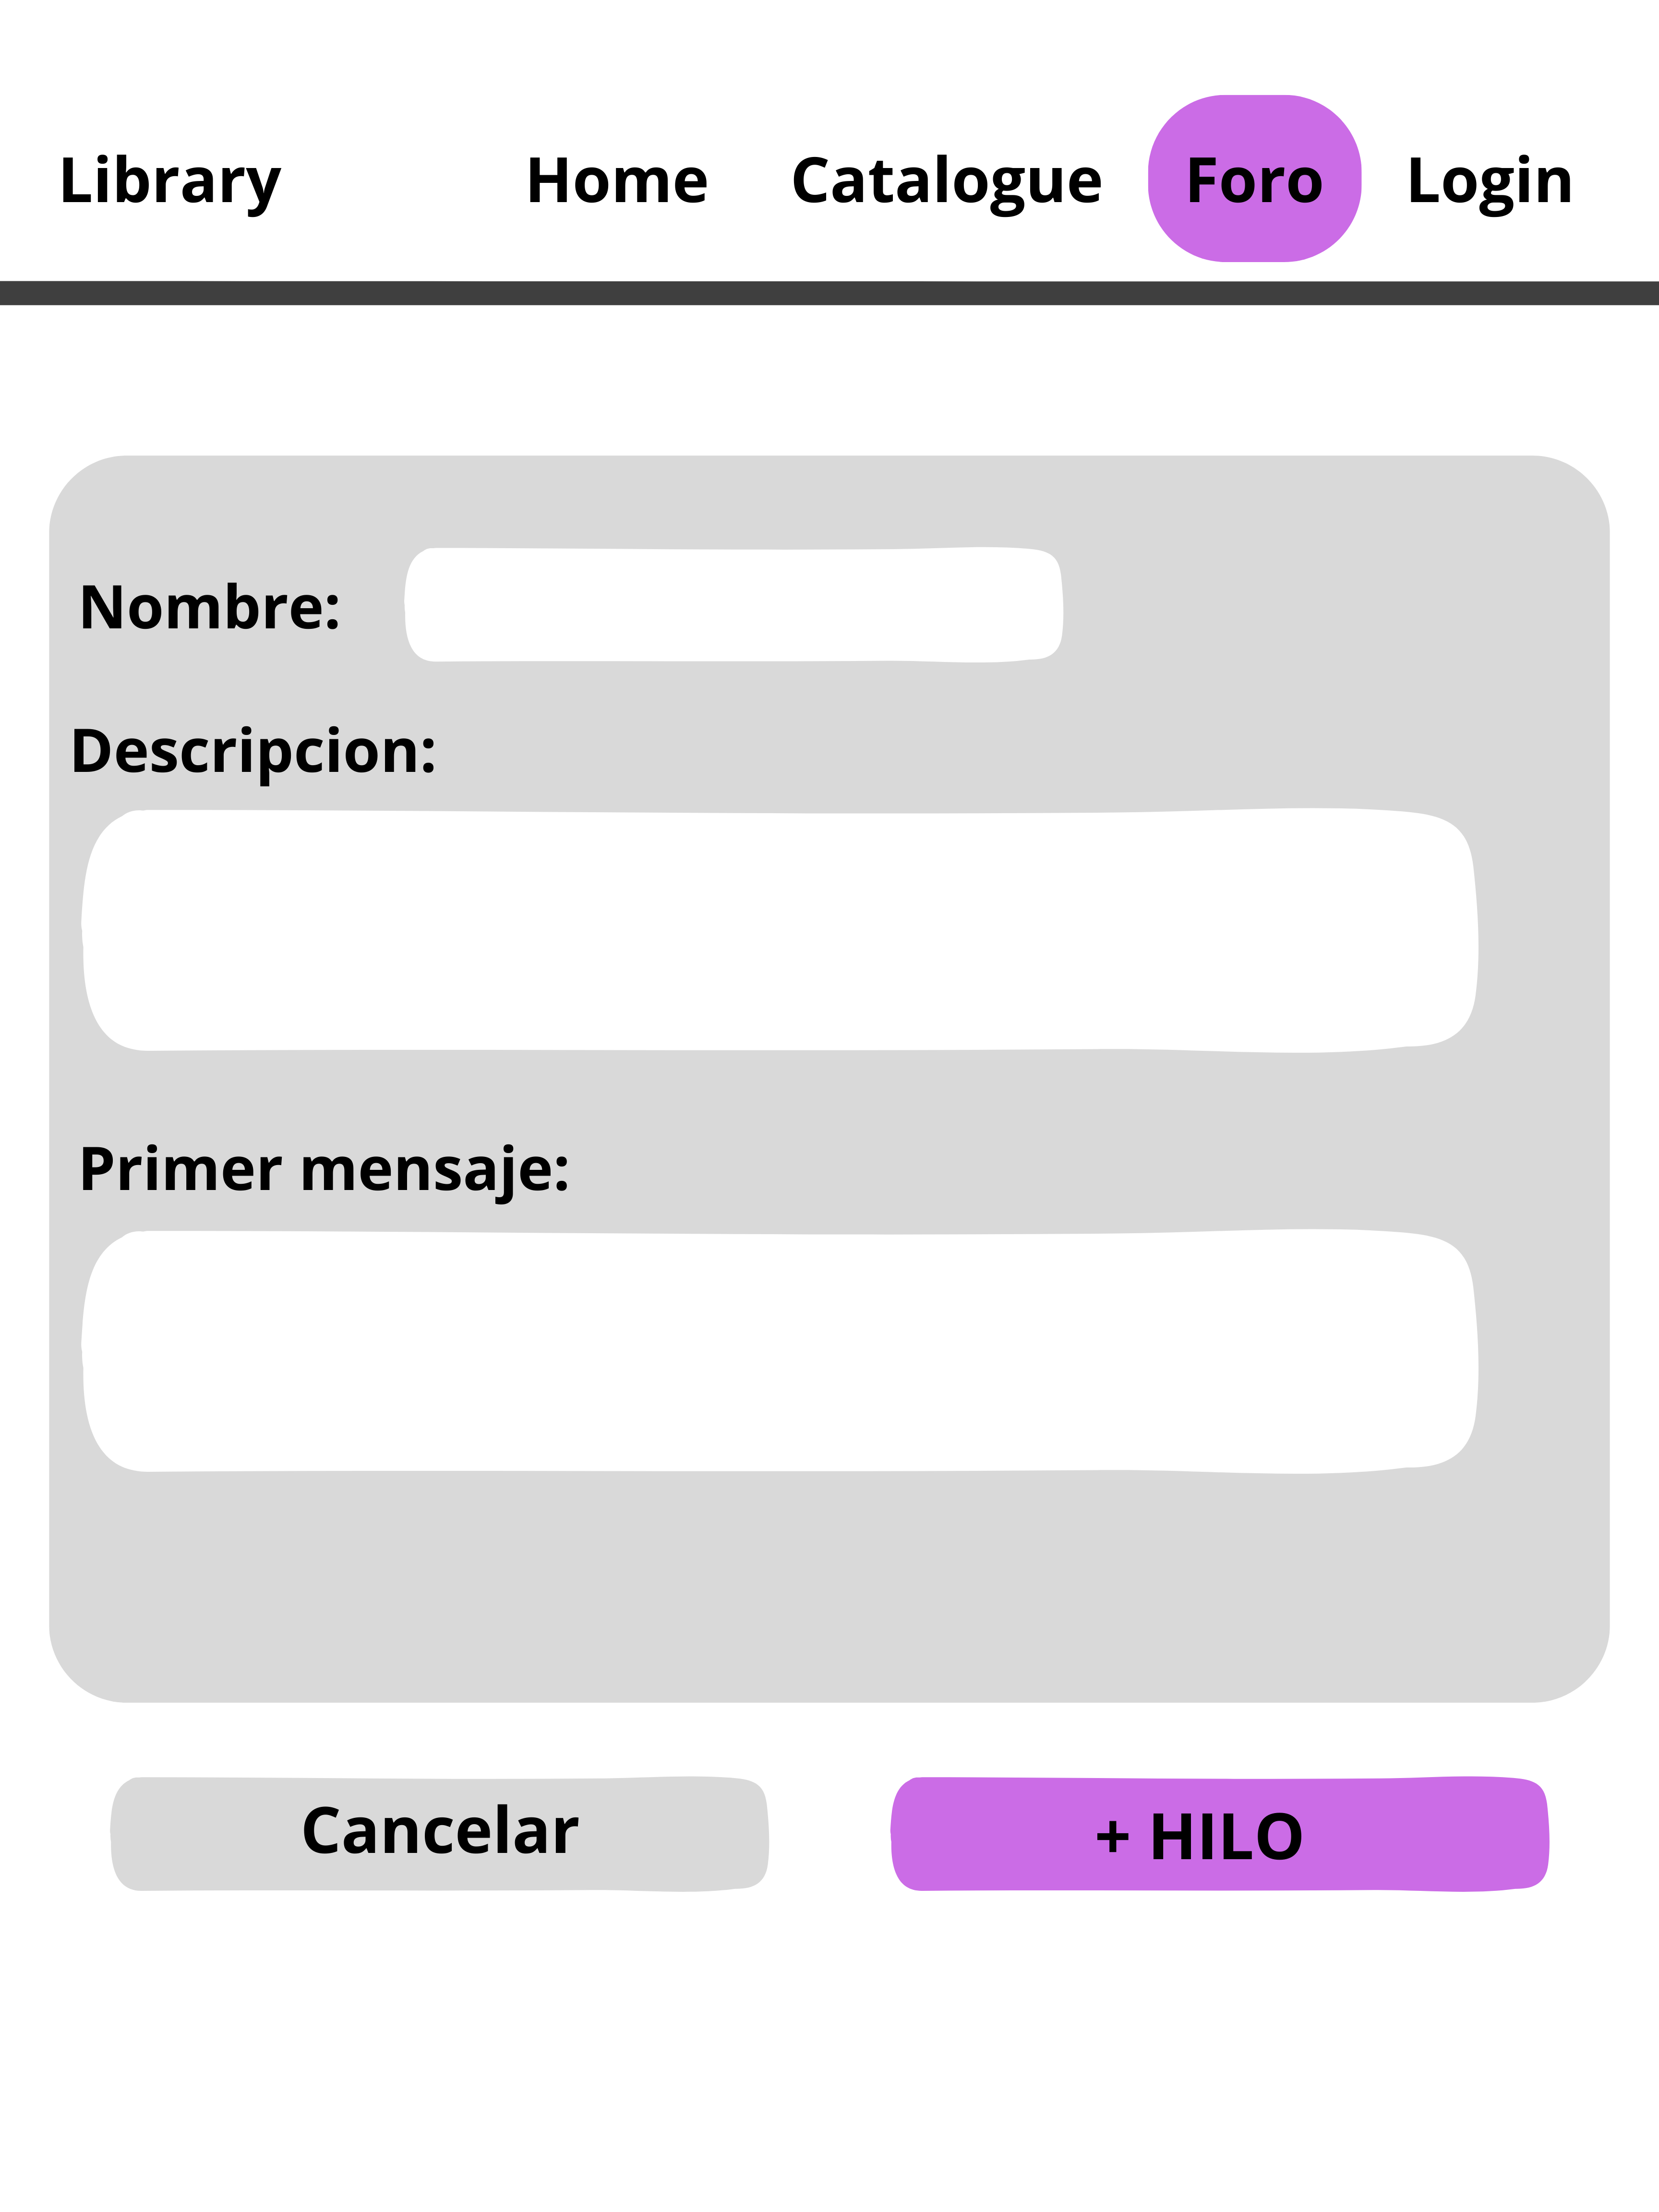
\includegraphics[width=0.8\textwidth]{./img/grafico/Foro2.png}
                            \\Figura 3.2.5.3: Interfaz para crear un hilo del foro.
                        \end{figure}\\
                        \begin{figure}[H]
                            \centering
                            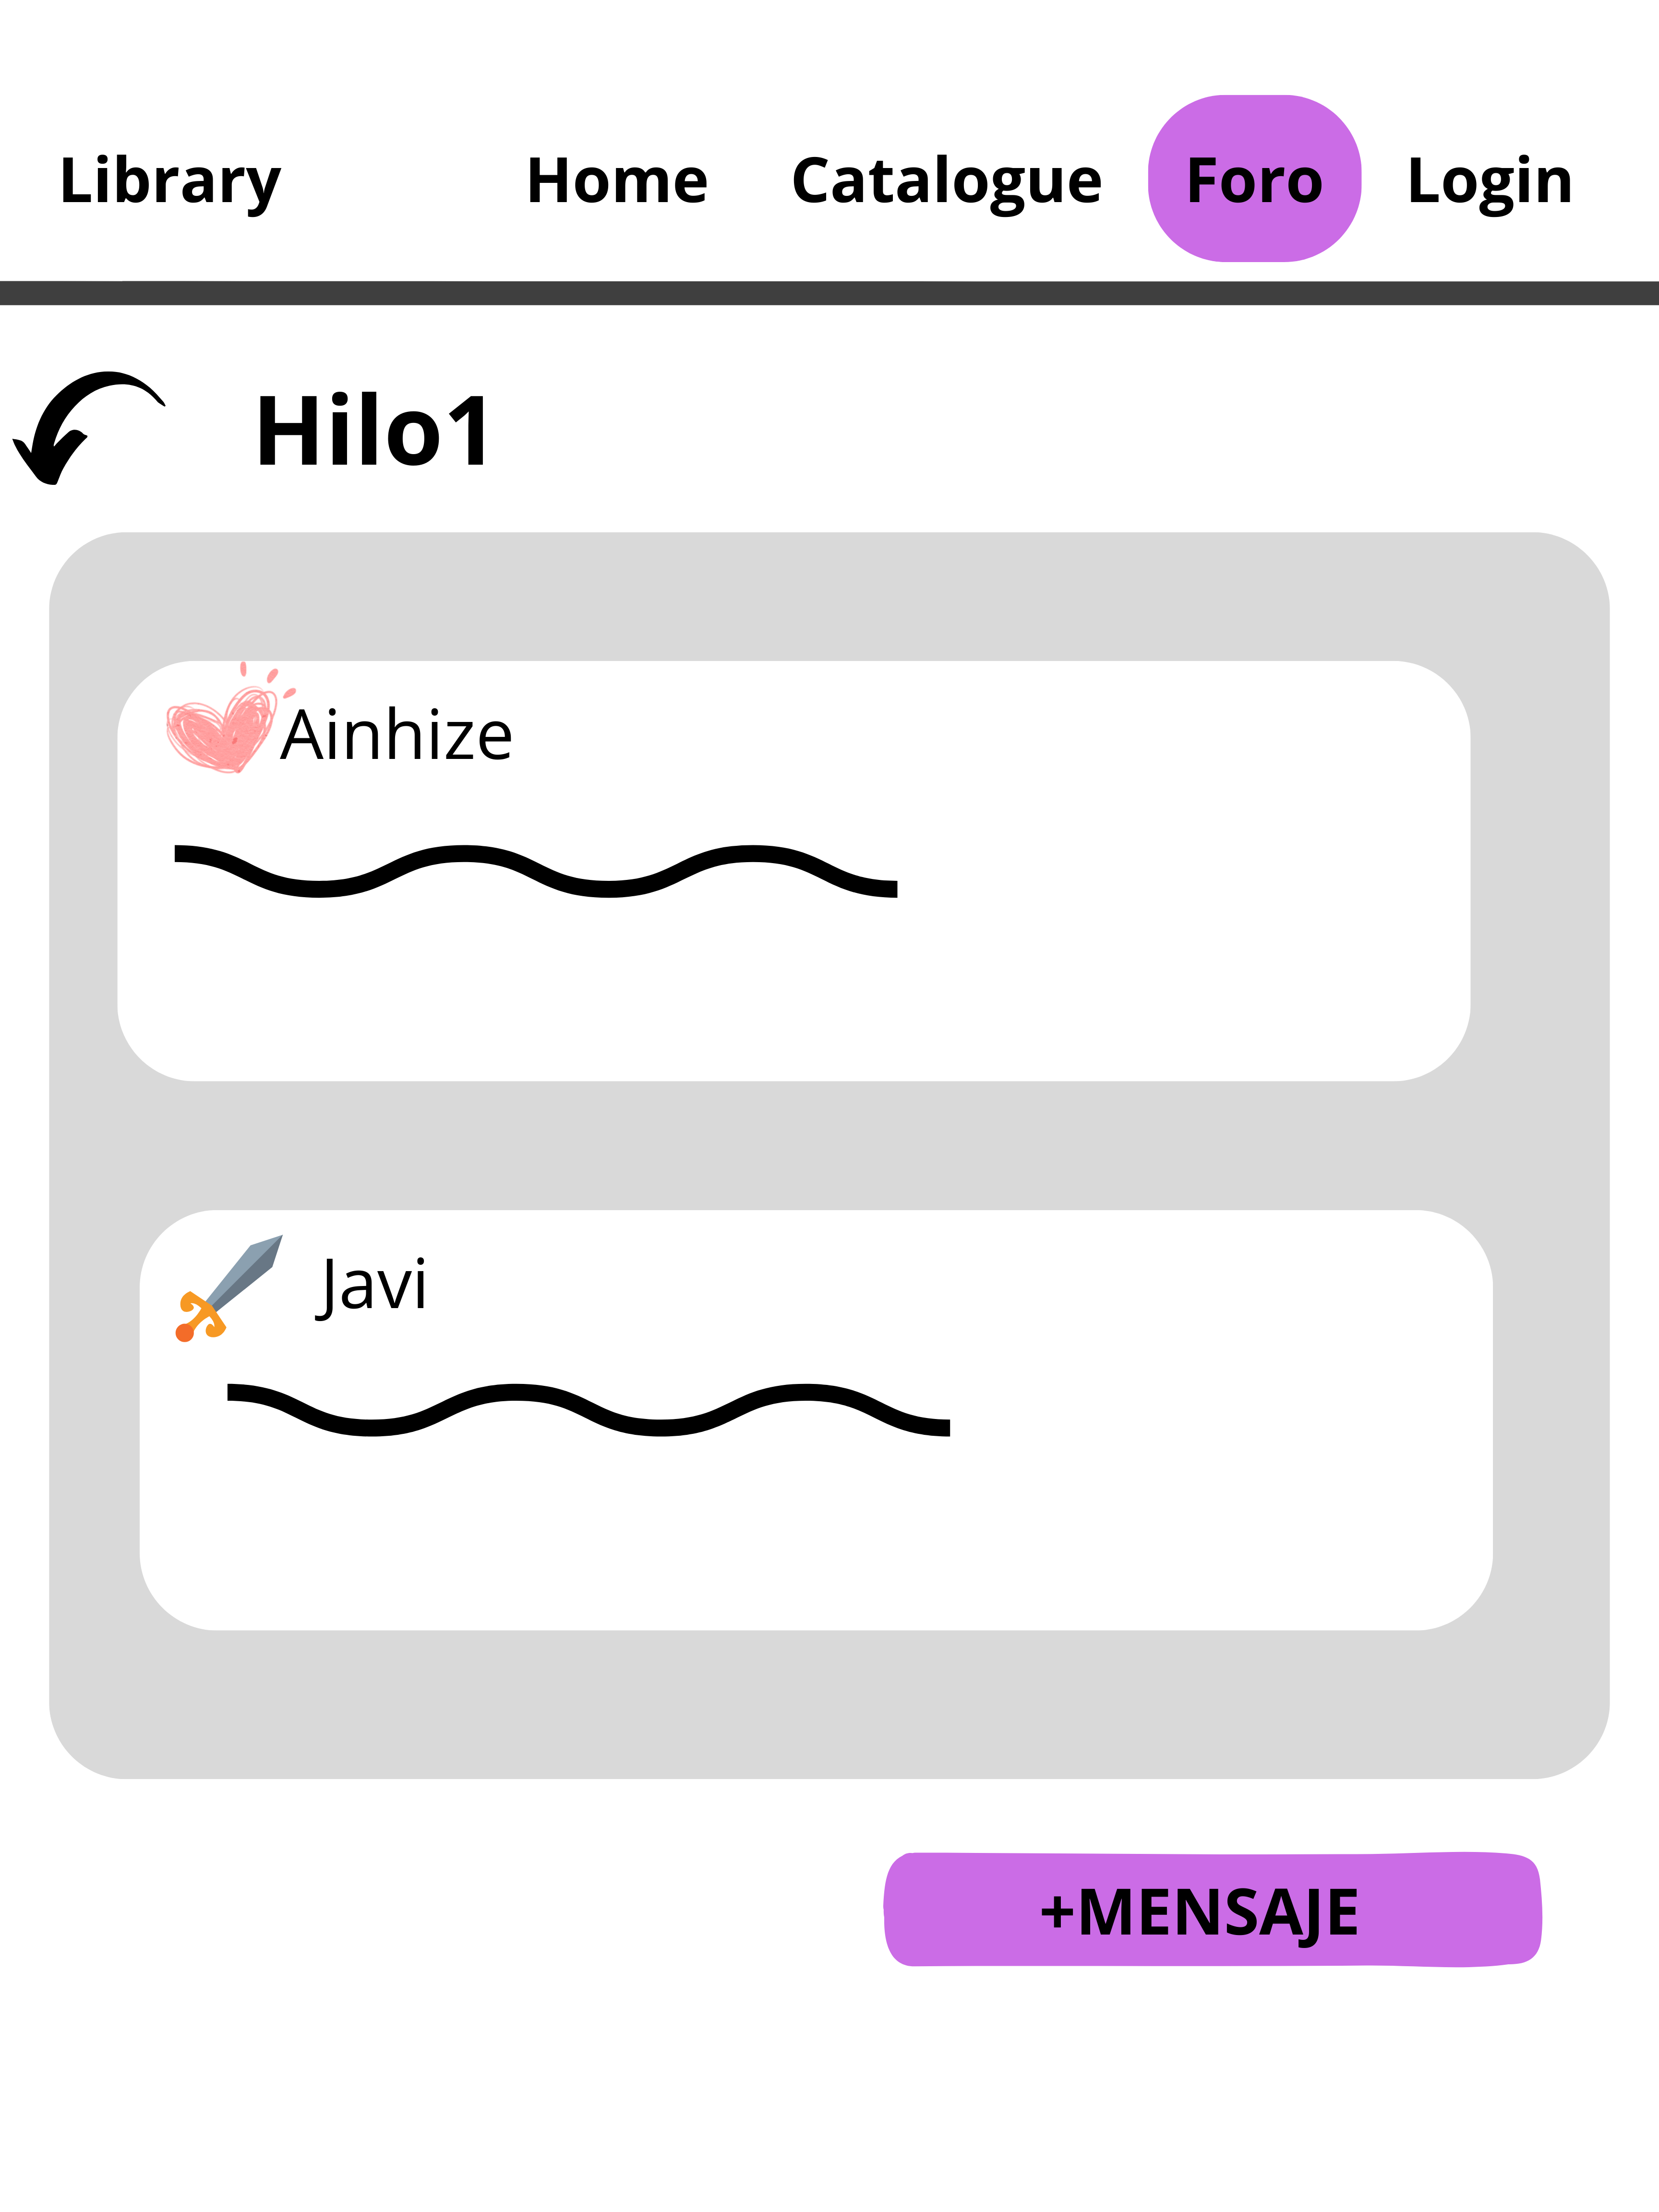
\includegraphics[width=0.8\textwidth]{./img/grafico/Foro3.png}
                            \\Figura 3.2.5.4: Interfaz para ver un hilo del foro.
                        \end{figure}\\
                        \begin{figure}[H]
                            \centering
                            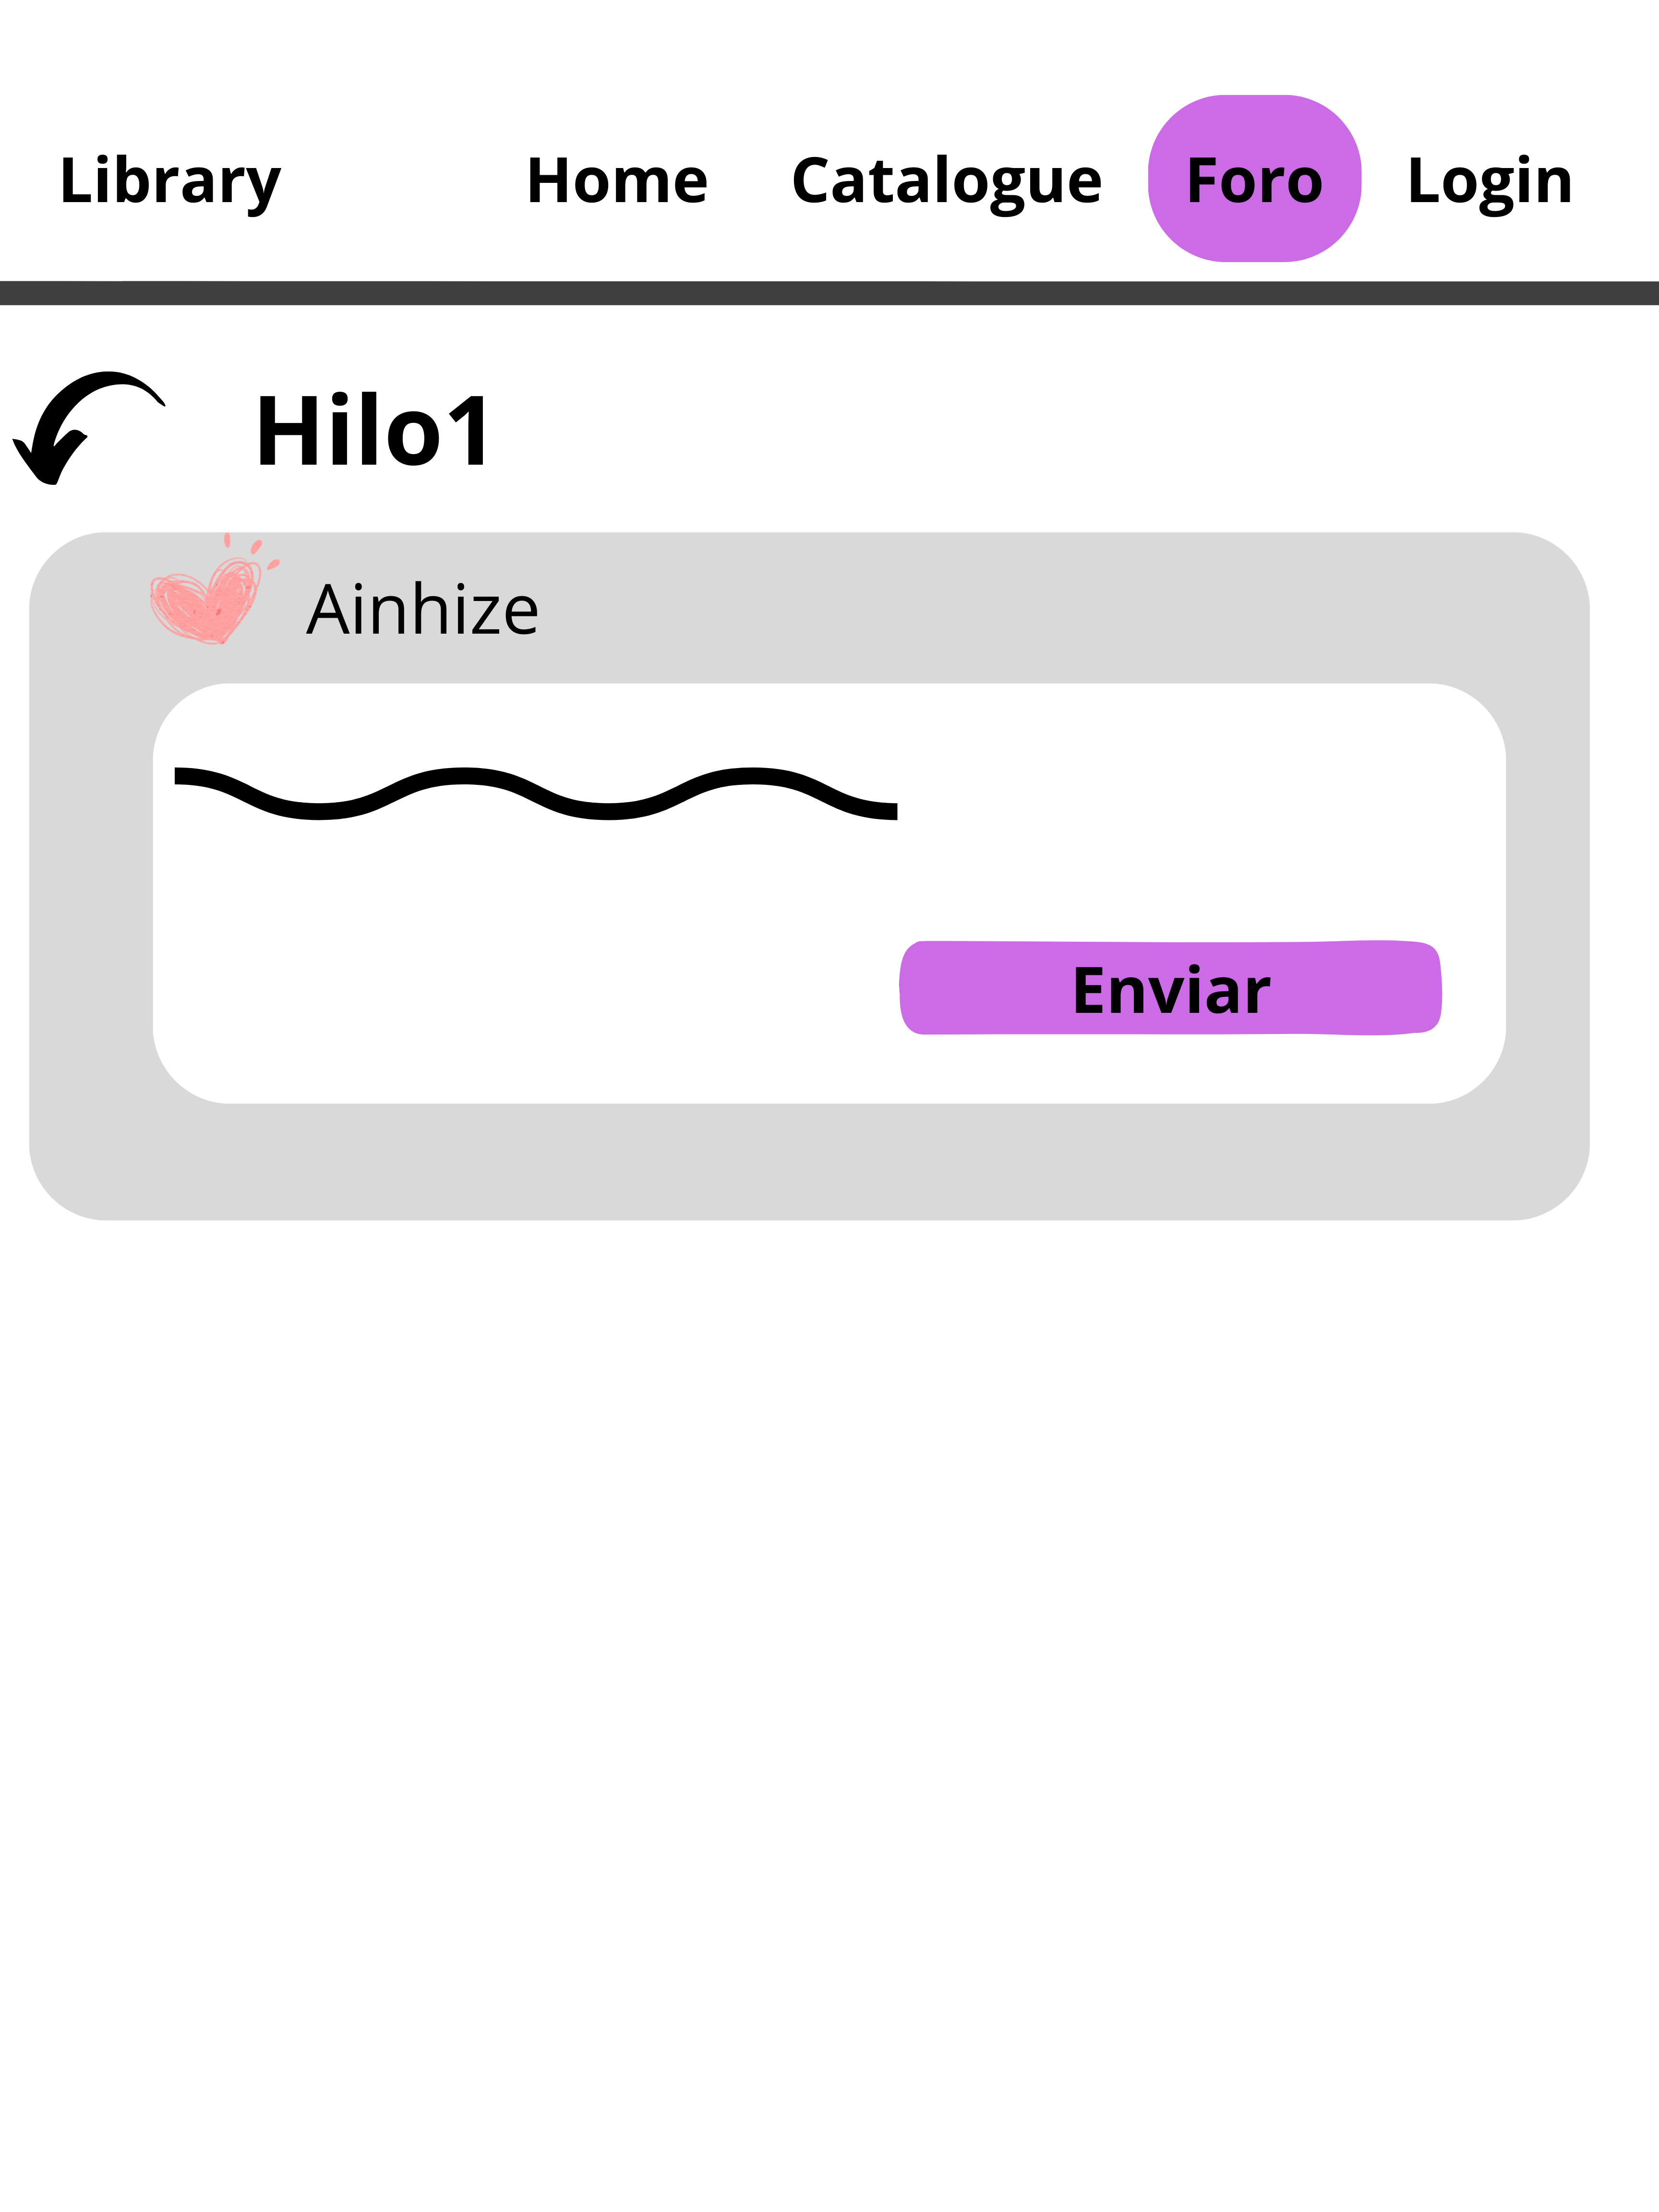
\includegraphics[width=0.8\textwidth]{./img/grafico/Foro4.png}
                            \\Figura 3.2.5.5: Interfaz para responder a un hilo.
                        \end{figure}\\
                        \hline
                    \end{longtable}
                \end{center}
                \clearpage
            \subsection{Recomendaciones del sistema}
                \begin{center}
                    \begin{longtable}{|p{\linewidth}|}
                        \hline
                        \textbf{Responsable:} Xabier Gabiña\\
                        \hline
                        \begin{figure}[H]
                            \centering
                            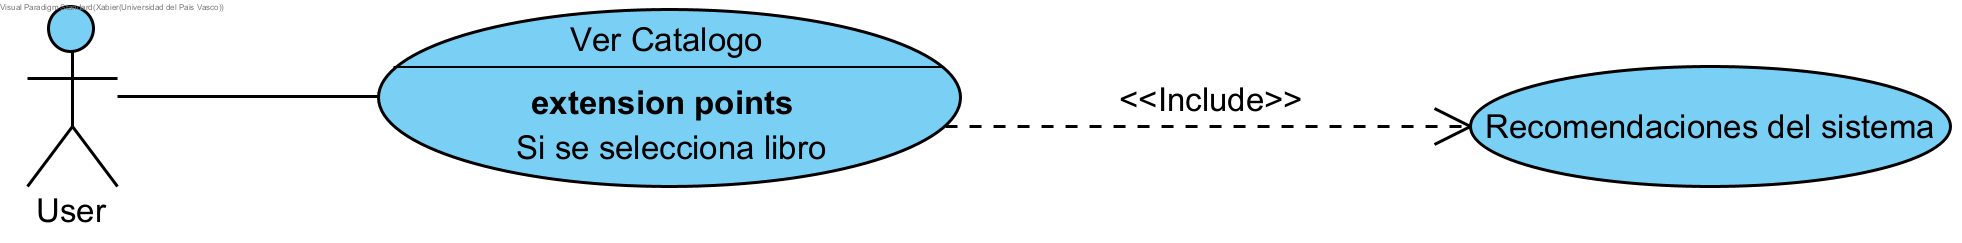
\includegraphics[width=0.8\textwidth]{./img/casos_uso/RecomendacionesLibros.png}
                            \\Figura 3.2.6.1: Diagrama de casos de uso de la subfuncionalidad de recomendaciones de libros
                        \end{figure}\\
                        \hline
                        \textbf{Nombre:} Recomendaciones del sistema\\
                        \hline
                        \textbf{Descripción:} Muestra una lista en la parte superior del catálogo mostrando los libros con más préstamos del sistema en funcion de los gustos del usuario.\\
                        \hline
                        \textbf{Actores:} Usuario\\
                        \hline
                        \textbf{Precondiciones:} Estar identificado en el sistema y haber tenido un libro reservado\\
                        \hline
                        \textbf{Requisitos no funcionales:} Ninguno\\
                        \hline
                        \textbf{Flujo de Eventos:}
                        \begin{enumerate}
                            \item El usuario entra en el catalogo para ver los libros disponibles.
                            \begin{enumerate}
                                \item Se le muestra en la parte superior de la pantalla una serie de libros basadas en los generos y peliculas que consume el usuario. [Figura 3.2.6.2]
                            \end{enumerate}
                        \end{enumerate}\\
                        \hline
                        \textbf{Poscondiciones:} Ninguna\\
                        \hline
                        \textbf{Interfaz Gráfica:}\\
                        \begin{figure}[H]
                            \centering
                            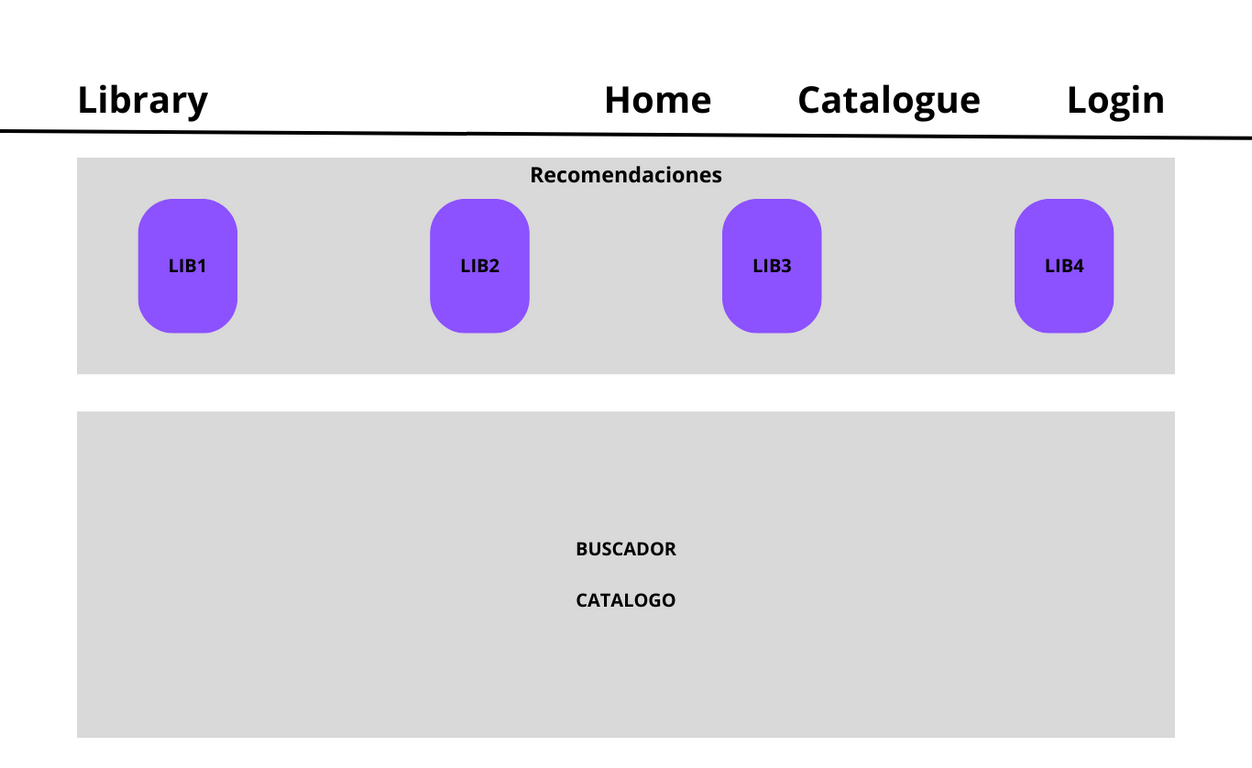
\includegraphics[width=0.8\textwidth]{./img/grafico/recom_lib.png}
                            \\Figura 3.2.6.2: Interfaz de recomendaciones de libros.
                        \end{figure}\\
                        \hline
                    \end{longtable}
                \end{center}
                \clearpage
            \subsection{Recomendaciones de amigos}
                \begin{center}
                    \begin{longtable}{|p{\linewidth}|}
                        \hline
                        \textbf{Responsable:} Kepa Reche\\
                        \hline
                        \begin{figure}[H]
                            \centering
                            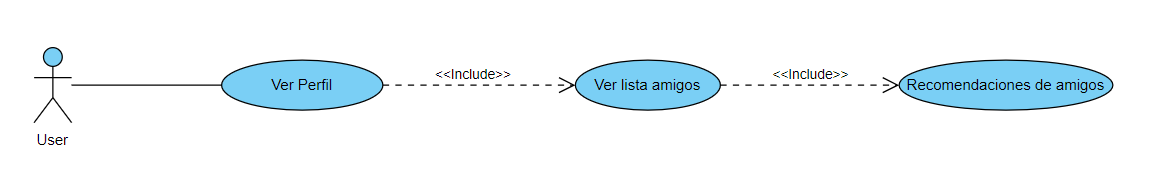
\includegraphics[width=0.8\textwidth]{./img/casos_uso/RecomendacionesAmigos.png}
                            \\Figura 3.2.7.1: Diagrama de casos de uso de la subfuncionalidad de recomendaciones de amigos
                        \end{figure}\\
                        \hline
                        \textbf{Nombre:} Ver amigos recomendados\\
                        \hline
                        \textbf{Descripción:} Muestra una lista en la parte superior de la lista de amigos mostrando posibles nuevos amigos basados en amigos de tus amigos o personas con las que tengas lecturas relacionadas.\\
                        \hline
                        \textbf{Actores:} Usuario\\
                        \hline
                        \textbf{Precondiciones:} Estar identificado en el sistema y tener algun amigo o libro guardado en tu perfil\\
                        \hline
                        \textbf{Requisitos no funcionales:} Ninguno\\
                        \hline
                        \textbf{Flujo de Eventos:}
                        \begin{enumerate}
                            \item El Usuario entra en su perfil.
                            \begin{enumerate}
                                \item Se le muestra en la parte superior de la lista de amigos varias personas recomendadas segun las lecturas en comun y amigos de amigos. [Figura 3.2.7.2]
                            \end{enumerate}
                        \end{enumerate}\\
                        \hline
                        \textbf{Poscondiciones:} Ninguna\\
                        \hline
                        \textbf{Interfaz Gráfica:}\\
                        \begin{figure}[H]
                            \centering
                            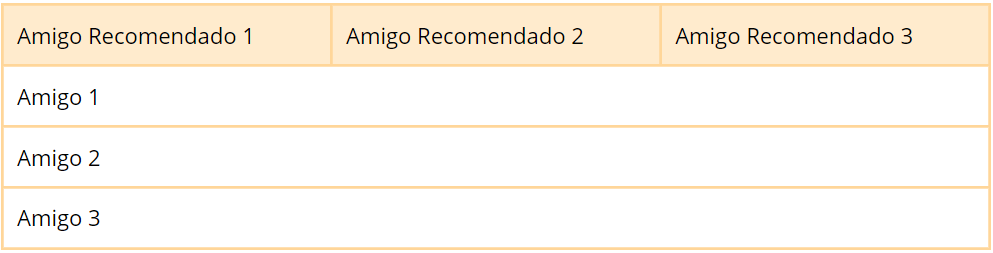
\includegraphics[width=0.8\textwidth]{./img/grafico/IU Recomendaciones de amigos.PNG}
                            \\Figura 3.2.7.2: Interfaz de recomendaciones de amigos.
                        \end{figure}\\
                        \hline
                    \end{longtable}
                \end{center}
                \clearpage
    \chapter{Modelo de Dominio}
        \section{Diagrama de modelo de dominio}
            \begin{figure}[H]
                \centering
                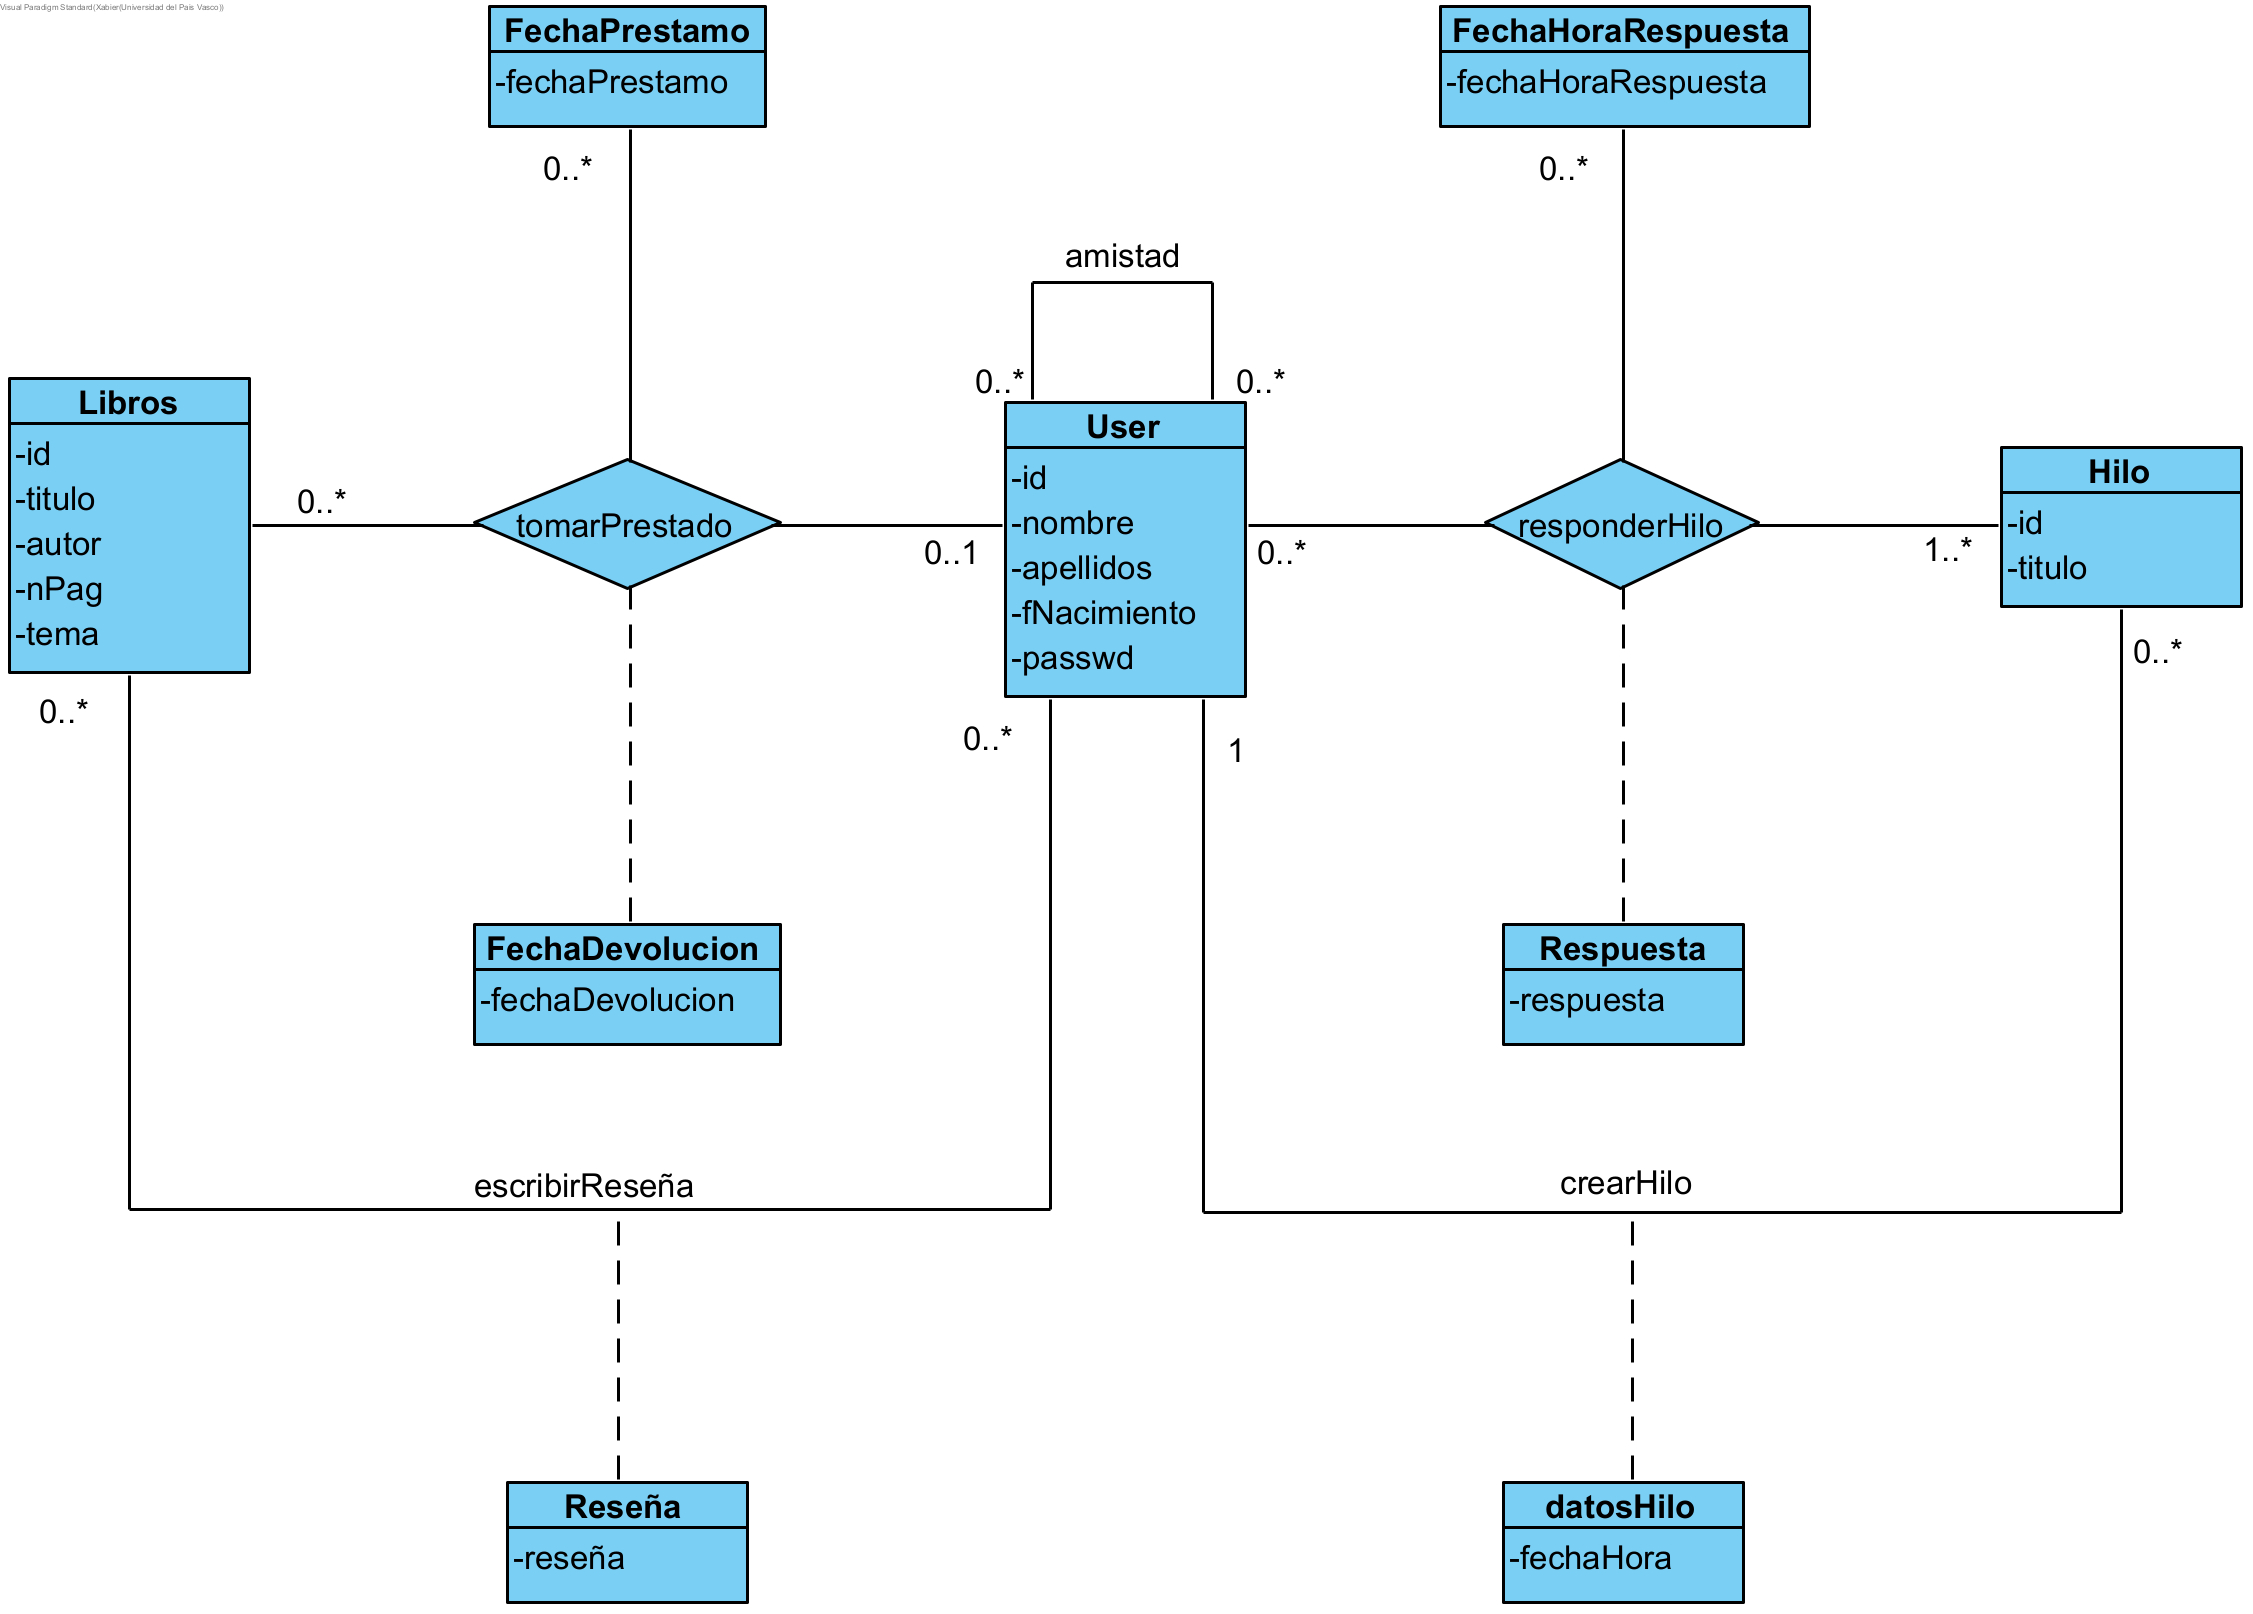
\includegraphics[width=1.0\textwidth]{img/dominio/Dominio.png}
                \caption{Diagrama de modelo de dominio}
            \end{figure}
        \clearpage
        \section{Desarrollo del modelo de dominio}
            \subsection{Entitades}
                \subsubsection{User}
                    La entidad usuario representa a los usuarios de la aplicacion. Dentro almacena sus datos personales como su id, nombre, apellidos, fecha de nacimiento...
                \subsubsection{Libros}
                    La entidad libro representa a los libros de la aplicacion. Dentro almacena sus datos como su id, titulo, autor, numero de paginas y genero.
                \subsubsection{FechaPrestamo}
                    La entidad fechaPrestamo representa a las fechas de prestamo de los libros. Sirve como clave para diferenciar los diferentes prestamos de un libro que puede hacer un usuario.
                \subsubsection{Hilo}
                    La entidad hilo representa a los hilos del foro. Dentro almacena la id del hilo y un titulo.
                \subsubsection{FechaHoraRespuestas}
                    La entidad fechaHoraRespuesta representa la fecha y hora en la que alguien ha dado una respuesta en el foro y sirve como clave para diferenciar del resto de respuestas que pueda dar un mismo usuario en un mismo hilo.
            \clearpage
            \subsection{Relaciones}
                \subsubsection{tomarPrestado}
                    Esta relacion es la que almacena los datos de los libros que se han tomado prestados y lo usuarios que los han tomado. La entidad fechaPrestamo es la encargada de diferencias las dos claves de usuario y libro y permitir asi que un usuario pueda tomar un mismo libro mas de una vez. El atributo de FechaDevolucion unicamente almacena como dato en la relacion la fecha en la que se devuelve el libro.
                    \begin{figure}[H]
                        \centering
                        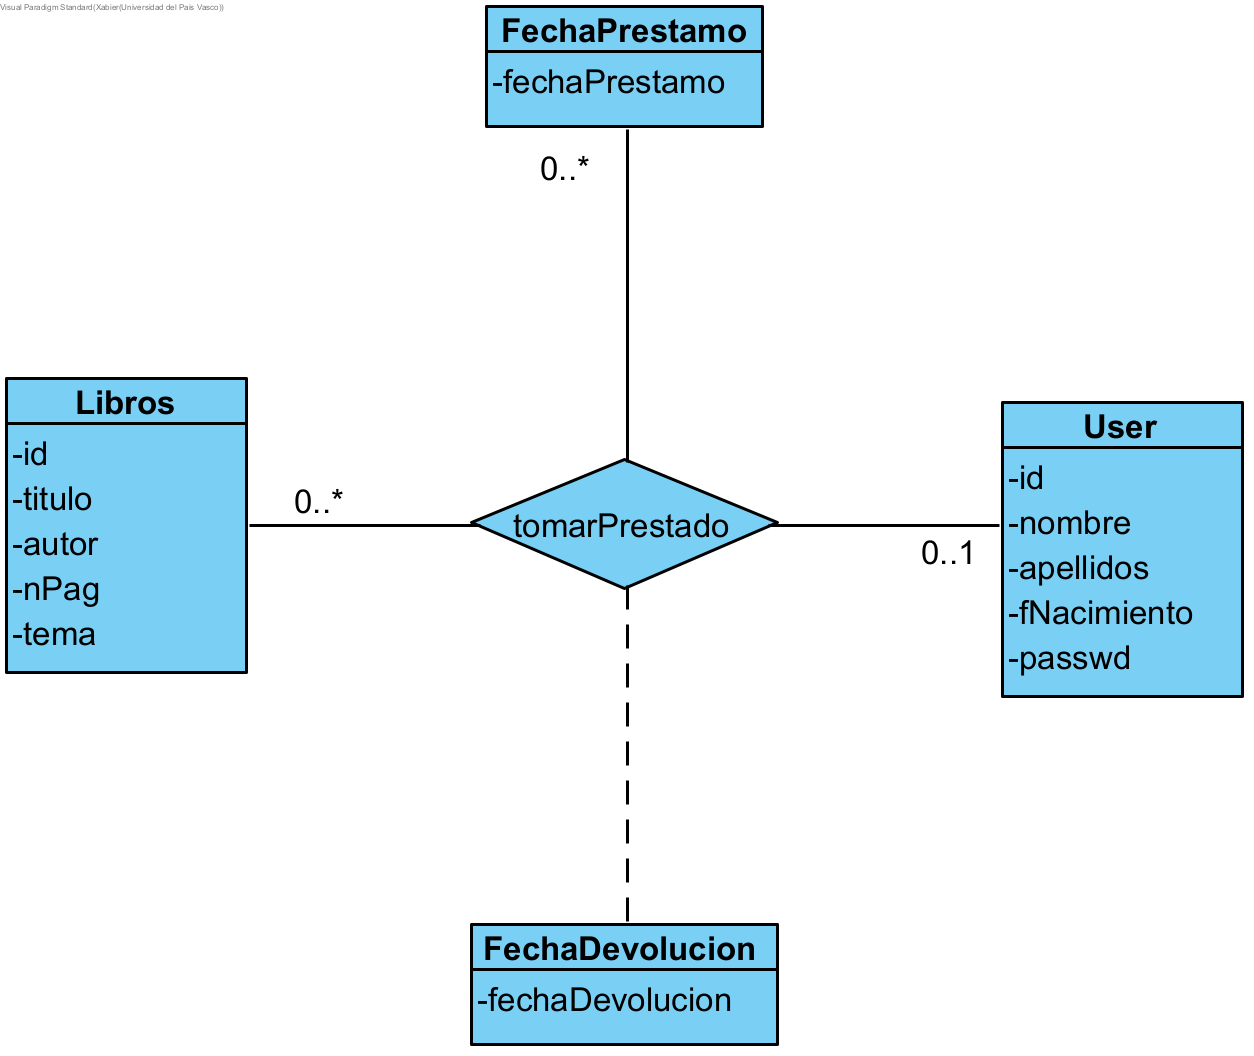
\includegraphics[width=1.0\textwidth]{img/dominio/tomarPrestado.png}
                        \caption{Diagrama de modelo de dominio de la relación tomarPrestado}
                    \end{figure}
                \clearpage
                \subsubsection{escribirReseña}
                    Esta relacion es la que permite guardar la reseña que un usuario pueda escribir en un libro. Al solo tener el atributo Reseña el usuario solo puede escribir una unica reseña sobre un libro.
                    \begin{figure}[H]
                        \centering
                        \includegraphics[width=1.0\textwidth]{img/dominio/escribirReseña.png}
                        \caption{Diagrama de modelo de dominio de la relación escribirReseña}
                    \end{figure}
                \clearpage
                \subsubsection{amistad}
                    La relacion amistad es la que permite que los usuarios puedan tener amigos en el sistema y guardar dichas amistades. 
                    \begin{figure}[H]
                        \centering
                        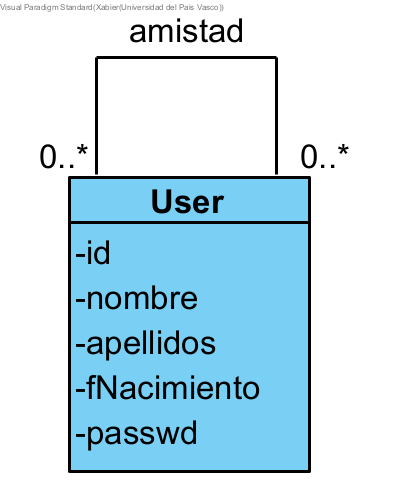
\includegraphics[width=0.5\textwidth]{img/dominio/amistad.png}
                        \caption{Diagrama de modelo de dominio de la relación amistad}
                    \end{figure}
                \clearpage
                \subsubsection{responderHilo}
                    Esta relacion permite que los usuarios puedan responder a los hilos del foro. La entidad fechaHoraRespuesta es la encargada de diferenciar las respuestas de un mismo usuario en un mismo hilo.
                    \begin{figure}[H]
                        \centering
                        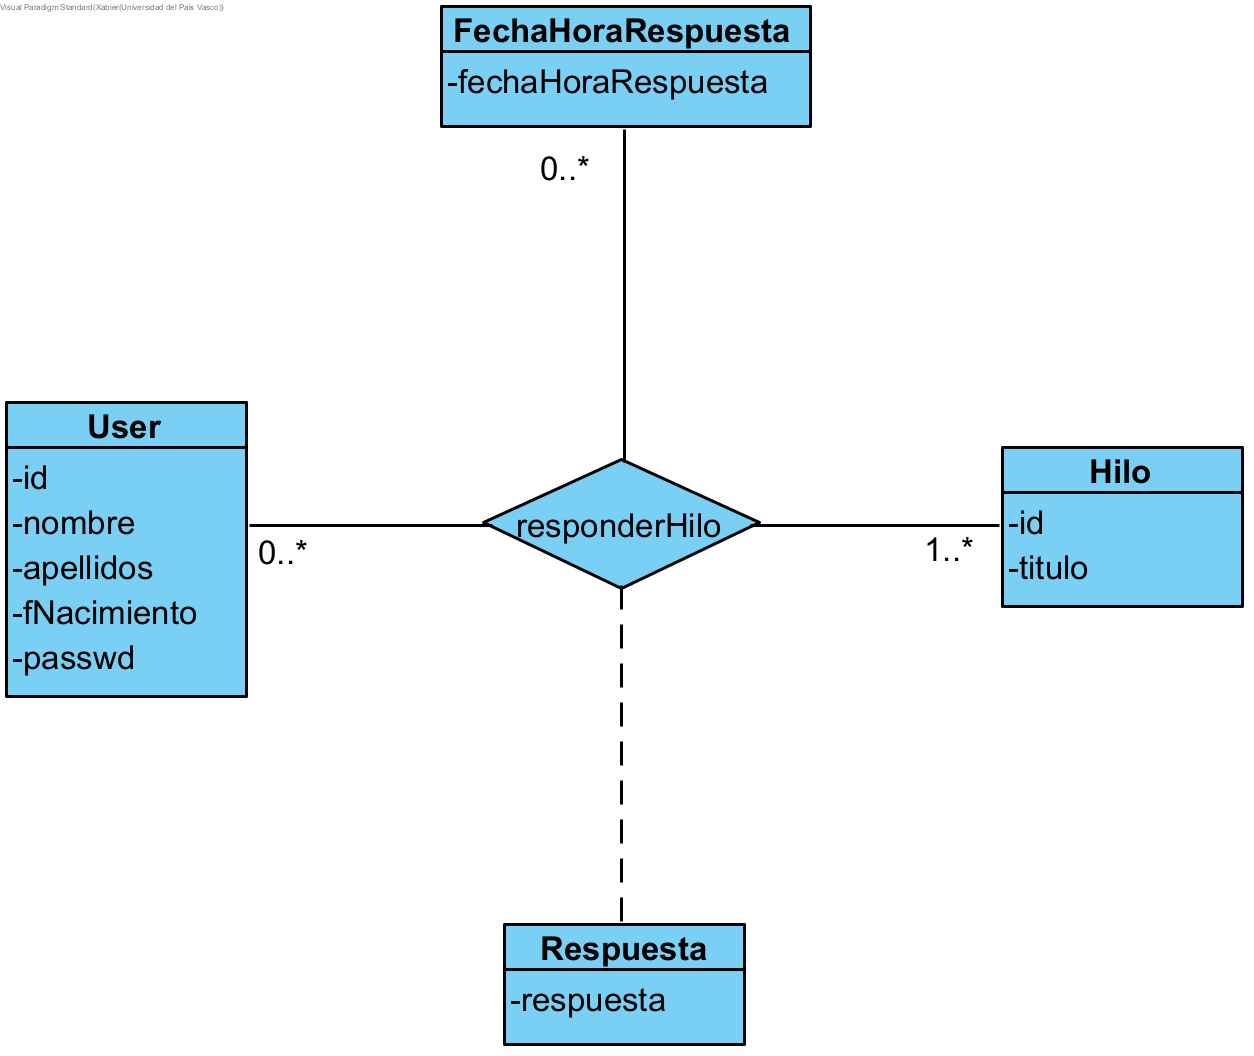
\includegraphics[width=1.0\textwidth]{img/dominio/responderHilo.png}
                        \caption{Diagrama de modelo de dominio de la relación responderHilo}
                    \end{figure}
                \clearpage
                \subsubsection{crearHilo}
                    Esta relacion almacena los datos de creacion de un hilo en el sistema. El sistema guardara el usuario que crea el hilo y en que fecha lo crea. Los hilos son unicos y para evitar repeticiones hacemos que sean unicos por lo que no guardamos la fecha como entidad si no como atributo de la relacion.
                    \begin{figure}[H]
                        \centering
                        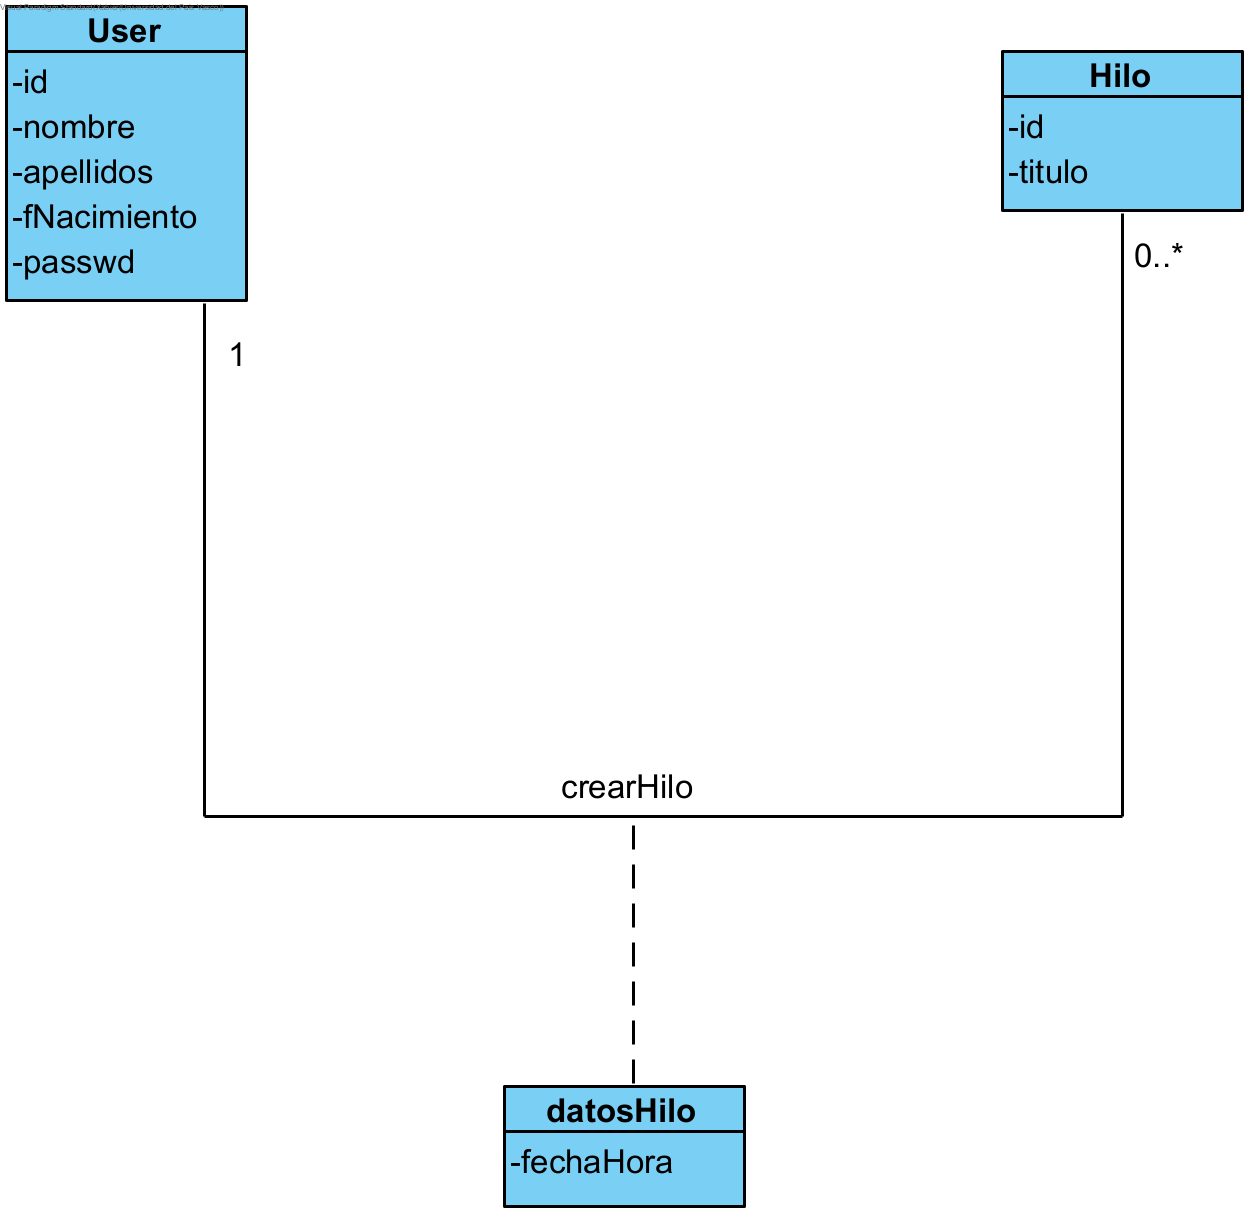
\includegraphics[width=0.7\textwidth]{img/dominio/crearHilo.png}
                        \caption{Diagrama de modelo de dominio de la relación crearHilo}
                    \end{figure}
\end{document}
